\documentclass{article}
\usepackage[12pt]{extsizes}
\usepackage[utf8]{inputenc}
\usepackage[T1,T2A]{fontenc}
\usepackage[english,russian]{babel}
\usepackage{setspace,amsmath}
\usepackage{enumitem}
\usepackage{etoolbox}
\usepackage[usenames, dvipsnames]{color}
\usepackage[left=30mm, top=20mm, right=20mm, bottom=20mm, footskip=10mm]{geometry}
\usepackage{amsmath}
\usepackage{amsfonts}
\usepackage{graphicx}
\usepackage{booktabs}
\usepackage{csquotes}
\usepackage{hyperref}
\usepackage{xcolor}
\usepackage{svg}
\usepackage{listings}
\usepackage{censor}

\usepackage[backend=biber]{biblatex}

\bibliography{main.bib}

\usepackage{setspace}
\onehalfspacing

\usepackage{mathptmx}

\begin{document}
% НАЧАЛО ТИТУЛЬНОГО ЛИСТА
\begin{center}

\small{ФЕДЕРАЛЬНОЕ ГОСУДАРСТВЕННОЕ АВТОНОМНОЕ ОБРАЗОВАТЕЛЬНОЕ УЧРЕЖДЕНИЕ ВЫСШЕГО ОБРАЗОВАНИЯ}\\
\footnotesize{НАЦИОНАЛЬНЫЙ ИССЛЕДОВАТЕЛЬСКИЙ УНИВЕРСИТЕТ}\\ 
\small{\textbf{ВЫСШАЯ ШКОЛА ЭКОНОМИКИ}}\\
\hfill \break
\hfill \break
\hfill \break
\hfill \break
\hfill \break
\hfill \break
\hfill \break
\hfill \break
\hfill \break
\large{ОТЧЕТ ПО НАУЧНО-ИССЛЕДОВАТЕЛЬСКОЙ РАБОТЕ}\\
Решение проблемы фаз в кристаллографии \\
методами машинного обучения
\end{center}
\hfill \break
\hfill \break
\hfill \break
\normalsize{
\begin{tabular}{lp{6cm}l}
Студент & & \censor{Глубшев Артем Игоревич}\\\\
& & \censor{Факультет Химии}  \\\\
Группа & & \censor{БХМ192} \\\\
Научный руководитель  &  &\censor{к.х.н. Дмитриенко Артем Олегович}\\\\
\end{tabular}
}\\
\hfill \break
\hfill \break 
\hfill \break
\hfill \break
\hfill \break
\hfill \break
\begin{center} Москва 2020 \end{center}
\thispagestyle{empty}
\newpage
\tableofcontents
\newpage


\section{ВВЕДЕНИЕ}
Проблема восстановления фаз из интенсивностей преобразования Фурье, нерешаемая в общем слуае, является одной из центральных проблем рентгеноструктурного анализа. Существуют как экспериментальные, так и расчетные методы определения фаз рентгеновских отражений, хорошо работающие для малых молекул. Однако для крупных молекул такие методы работают плохо или не работают вообще\cite{PhaseProblem}. Также все существующие методы имеют невысокую точность и требуют участия человека в решении кристаллов, что затрудняет автоматизацию. Таким образом, задача разработки метода, способного без участия человека решать кристаллы с приемлемой точностью все еще актуальна. 

\section{ОБЗОР ЛИТЕРАТУРЫ}

Машинное обучение и нейронные сети в частности помогли решить множество проблем, ранее считавшиеся крайне сложными. В частности, с помошью методов машинного обучения была решена \cite{XRD-NN} задача классификации картин порошковой рентгеновской дифракции, определения параметров кристаллической решетки\cite{MCMC}. Также машинное обучение широко применяется в науке о материалах\cite{ML-mat}.

Актуальные методы решения проблемы фаз в рентгенструктурном анализе можно разделить на три типа: методы в прямом пространстве, методы в обратном пространстве, методы в ???(как по русски dual-space?)\cite{XR-ED}. Рассмотрим основные методы решения проблемы фаз.

\subsection{Метод Паттерсона}

Структура малых молекул может быть решена даже при отсутствии информации о фазах. В то время как фазы определяют положения пиков электронной плотности поперек элементарной ячейки и, следовательно, положения атомов, одно только сильное дифракционное пятно дает четкое указание на то, что элементы должны присутствовать с соответствующим интервалом. Таким образом, только величины структурного фактора содержат информацию о расположении атомов в структуре.

Доступ к этой информации можно получить, вычислив функцию Паттерсона\cite{PattersonMethod}. Функция Паттерсона получается путем расчета карты с использованием квадратов величин структурных факторов и всех фаз, установленных на ноль. Вместо пиков в положениях атомов карта Паттерсона показывает пики в каждой позиции, которая соответствует межатомному вектору в структуре. Функция Паттерсона была эффективным инструментом для решения проблем малых молекул; однако его полезность быстро падает с увеличением числа атомов. Для структуры из $N$ атомов функция Паттерсона будет содержать $N (N - 1)$ межатомных векторов, многие из которых перекрываются. Этот подход становится непригодным для структур из более чем 20–50 атомов, если не существует подмножества атомов с высоким атомный номер.



\section{ОСНОВНАЯ ЧАСТЬ}
Все модели обучались на суперкомпьютере НИУ ВШЭ <<Харизма>>. Для создания моделей использовался язык python и билиотеки машинного обучения Tensorflow и Keras. Все модели использовали бинарную кроссэнтропию, взвешенную по интенсивности отражения, в качестве функции ошибки и точность предсказаний в качестве метрики, если не указано иного.
  
\subsection{Получение данных. Датасеты}
Экспериментальные кристаллографические данные были получены из Acta Cristallographica Section E в виде cif-файлов. Данные были обработаны с помощью python и библиотек pandas и CCTBX для получения пригодного для обучения датасета: были отобраны отражения с индексами $h,k,l \in [-10, 10]$, удалены эквивалентные отражения(для группы $P-1$ эквивалентными являются отражения удовлетворяющие условию $h_1=-h_2, k_1=-k_2, l_1=-l_2$). Размер полученного датасета составил 7000 файлов - 6000 в обучающем датасете, 1000 в тестовом, по 4630 отражений в каждом. Проверка корректности расчета фаз отражений библиотекой cctbx была показана проверкой корреляции рассчетных интенсивностей с экспериментальными(рис. \ref{img:dist}). 

\begin{figure}[h!]
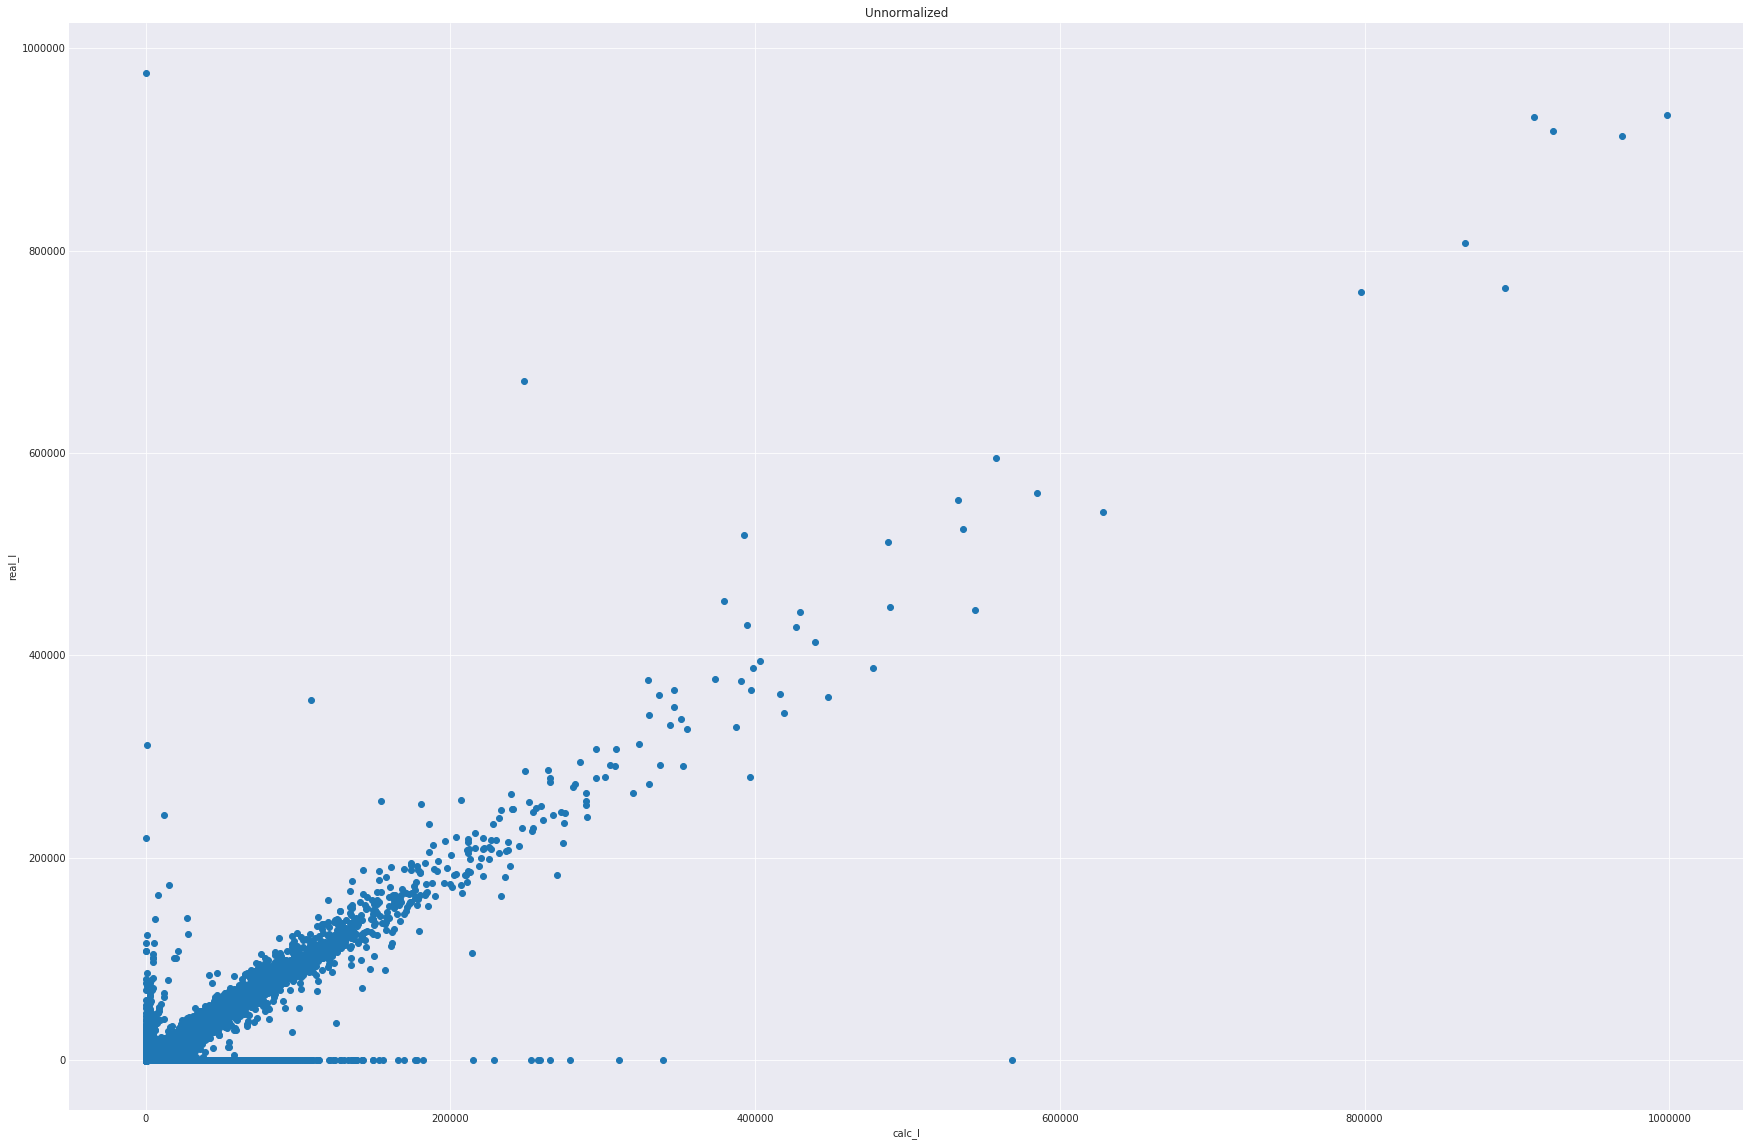
\includegraphics[width=\linewidth]{imgs/dist.png}
  \caption{Распределение реальных интенсивностей от рассчетных}\label{img:dist}
\end{figure}


 По итогам этой проверки стало ясно что интенсивности в файлах очень зависят от экспериментальных условий, а не только от структурных факторов - у каждого из файлов распределение $I_{exp}(I_{calc})$хорошо приближалось линейной регрессией, но коэффициенты $\frac{I_{exp}}{I_{calc}}$ сильно отличались для каждого из файлов. и чтобы исключить это влияние была необходима нормализация. Нормализация по максимуму (рис. \ref{fig:dist_max}), среднему (рис. \ref{fig:dist_mean} и медиане (рис. \ref{fig:dist_med} не дала результатов, и коэффициенты $\frac{I_{exp}}{I_{calc}}$ все так же сильно отличаются. Это может быть связано с далеким от нормального распределением значений структурных факторов.

\begin{figure}[!h]
\minipage{0.33\textwidth}%
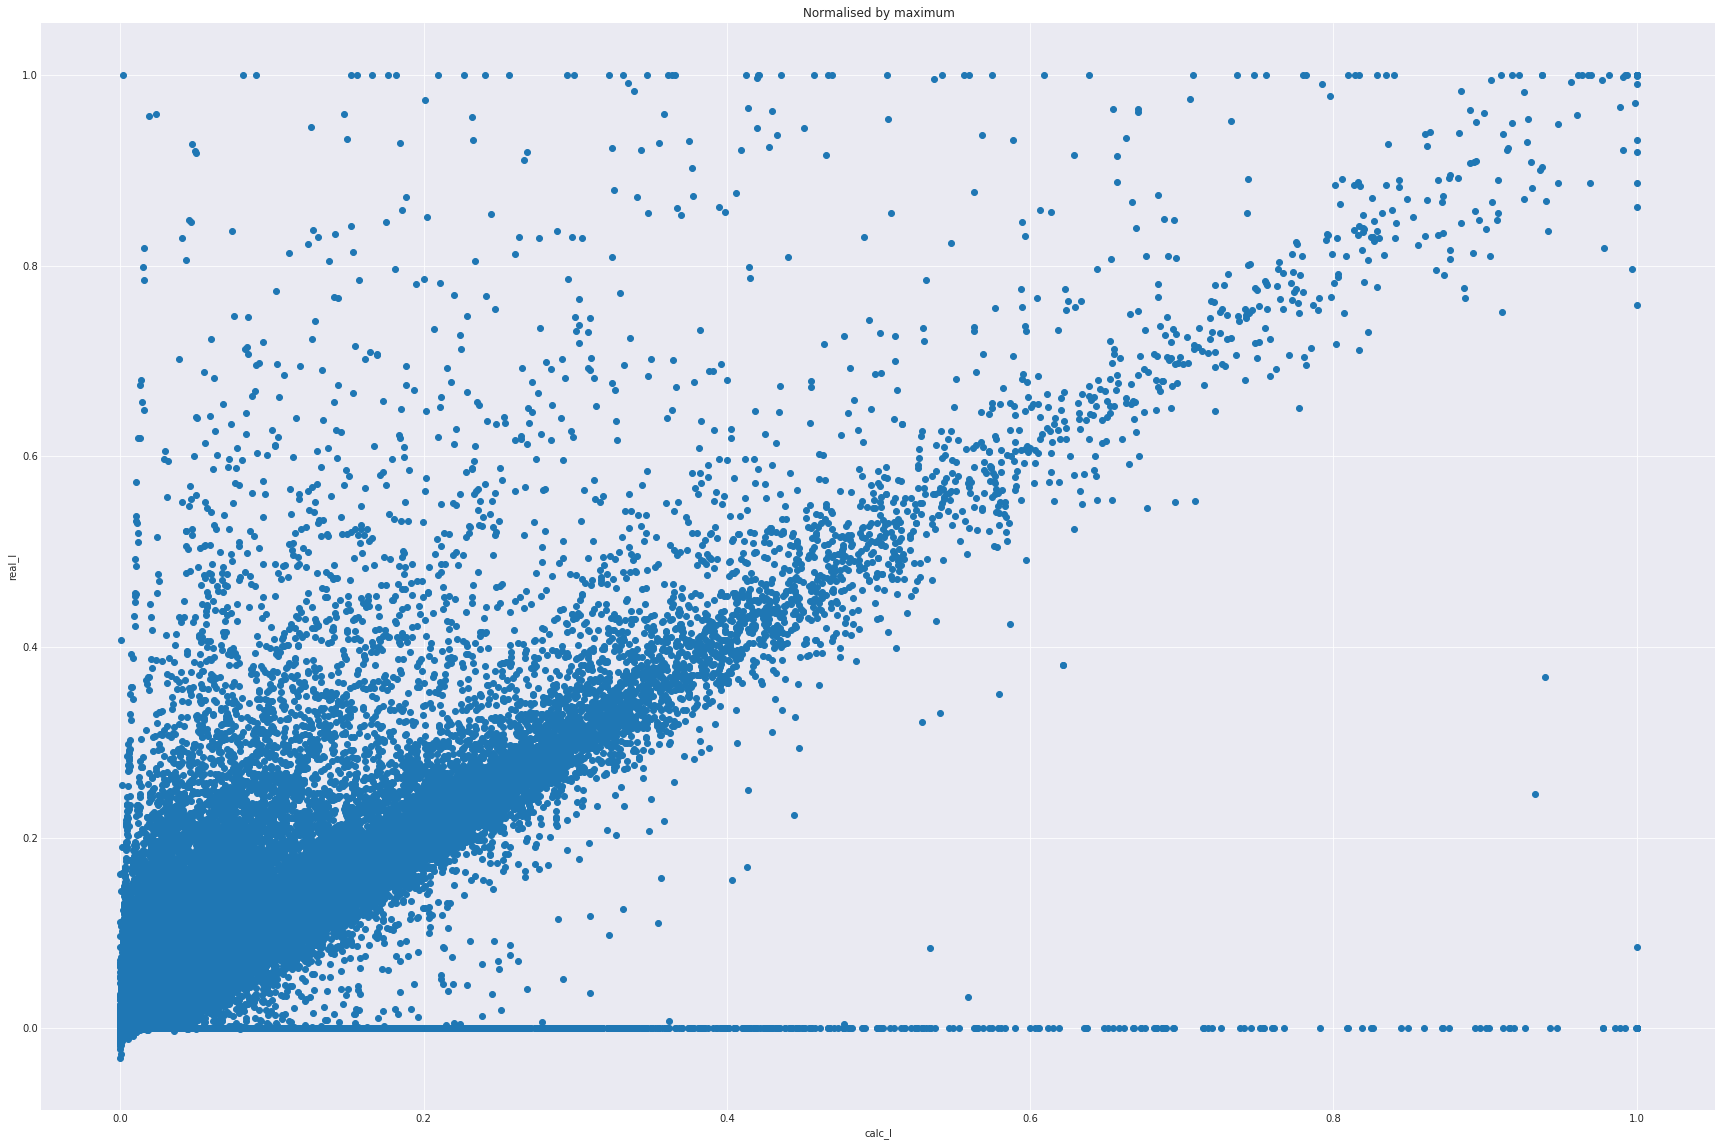
\includegraphics[width=\linewidth]{imgs/dist_max.png}
  \caption{нормализация по максимуму}\label{fig:dist_max}
\endminipage
\minipage{0.33\textwidth}%
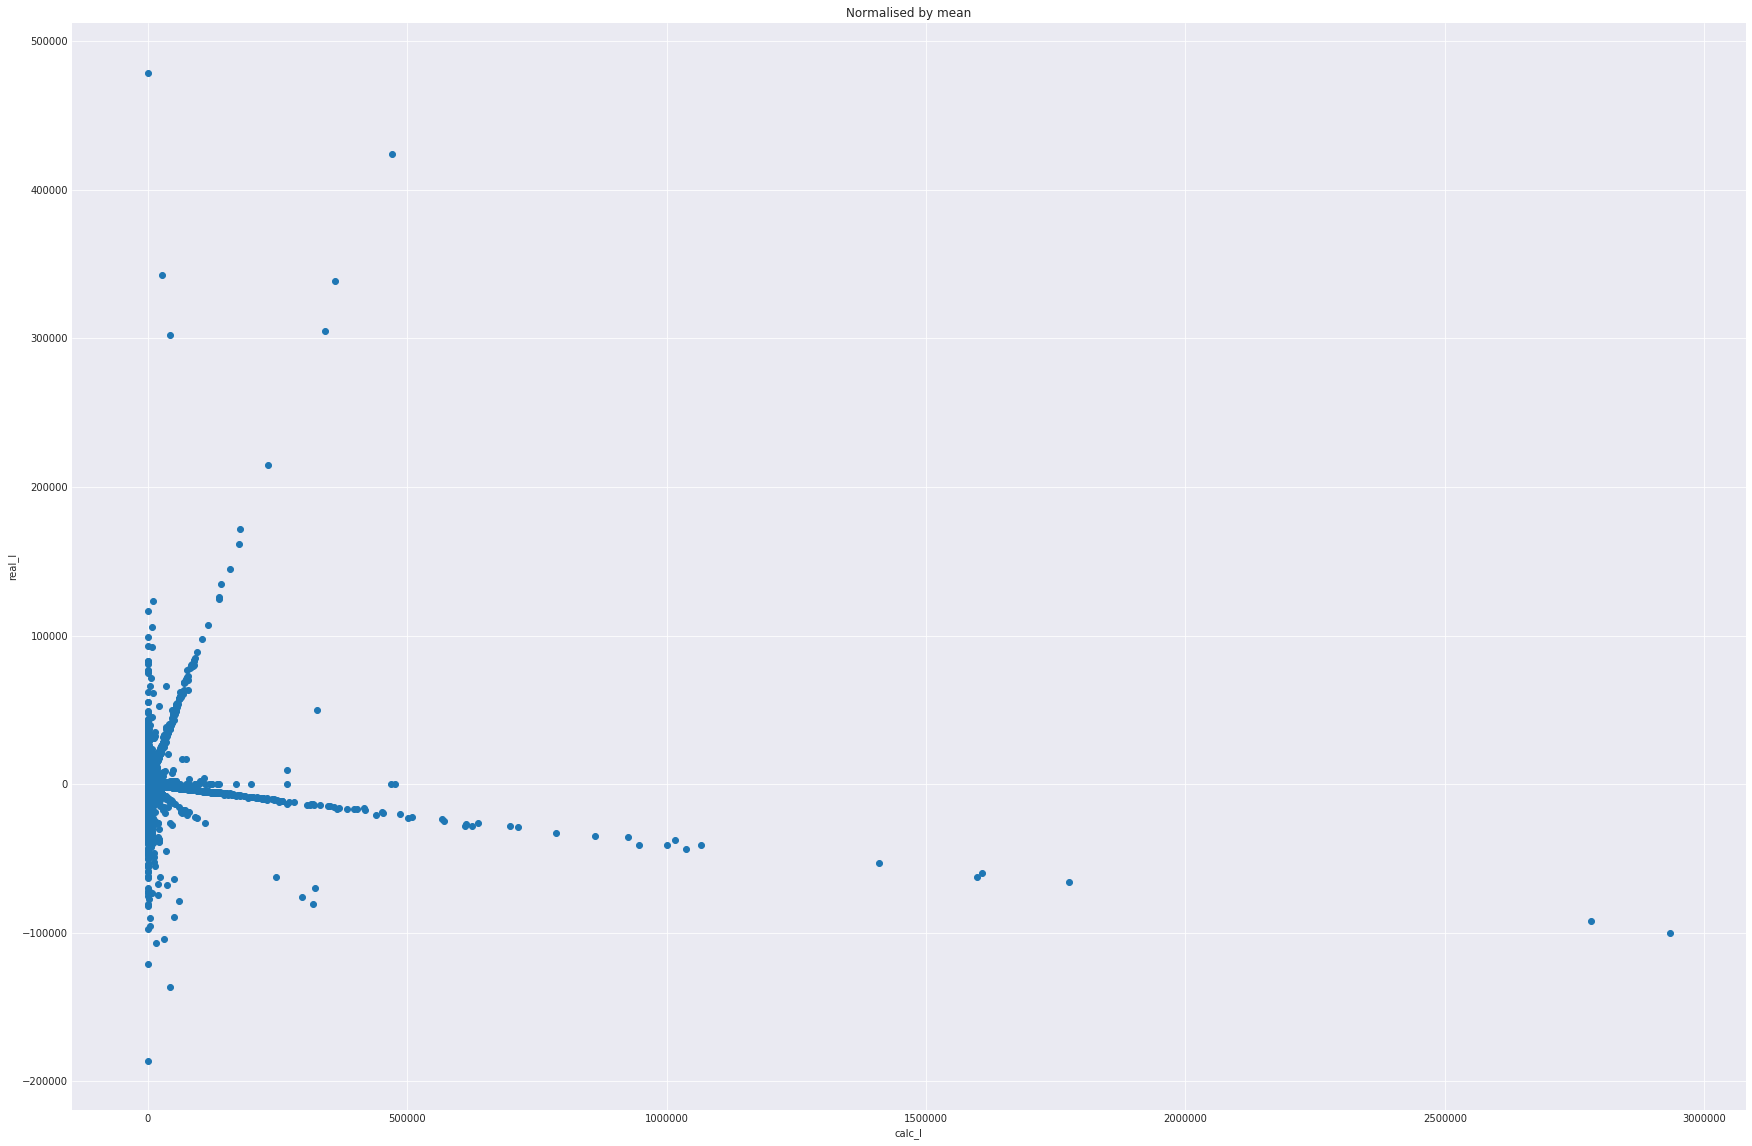
\includegraphics[width=\linewidth]{imgs/dist_mean.png}
  \caption{нормализация по среднему значению}\label{fig:dist_mean}
\endminipage
\minipage{0.33\textwidth}
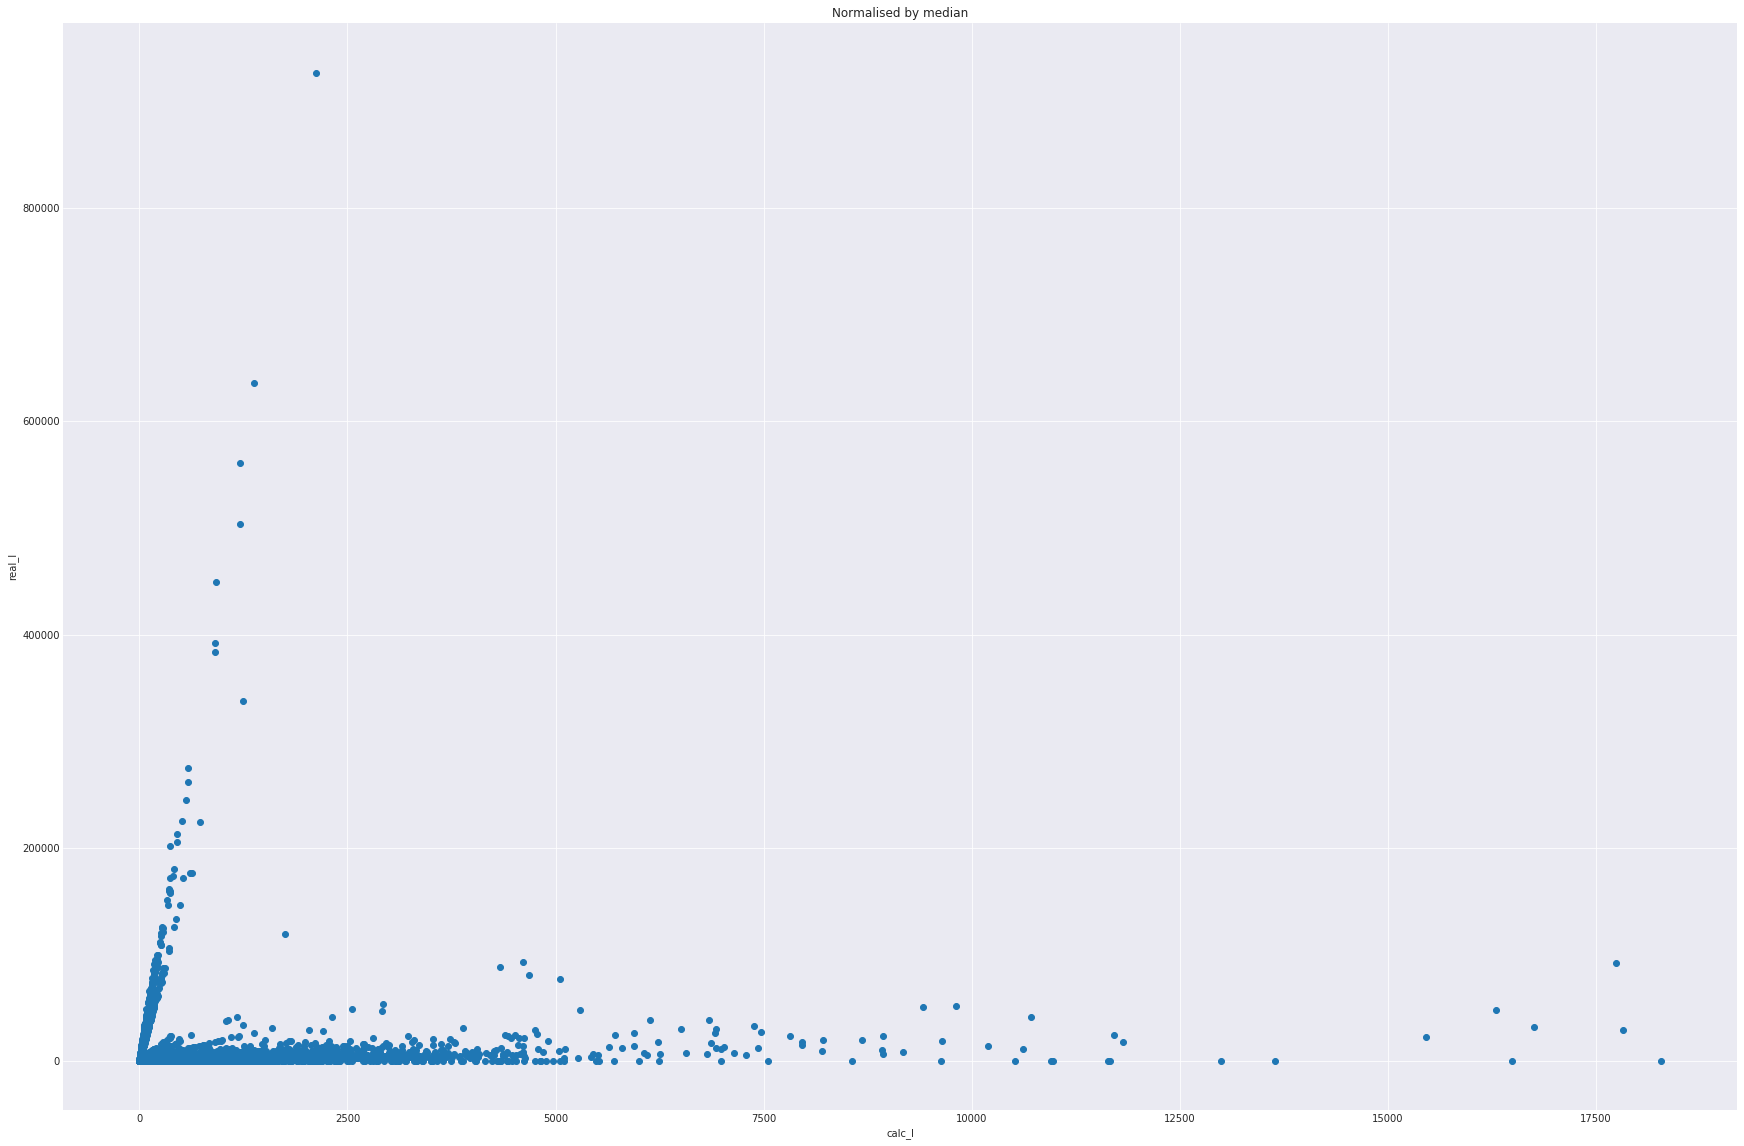
\includegraphics[width=\linewidth]{imgs/dist_med.png}
  \caption{Нормализация по медиане}\label{fig:dist_med}
\endminipage\hfill
\end{figure}

Лучший результат был получен при использовании линейной регрессии - все данные уложились близко к одной линии, что положительно влияет на качество работы НС.

\begin{figure}[h!]
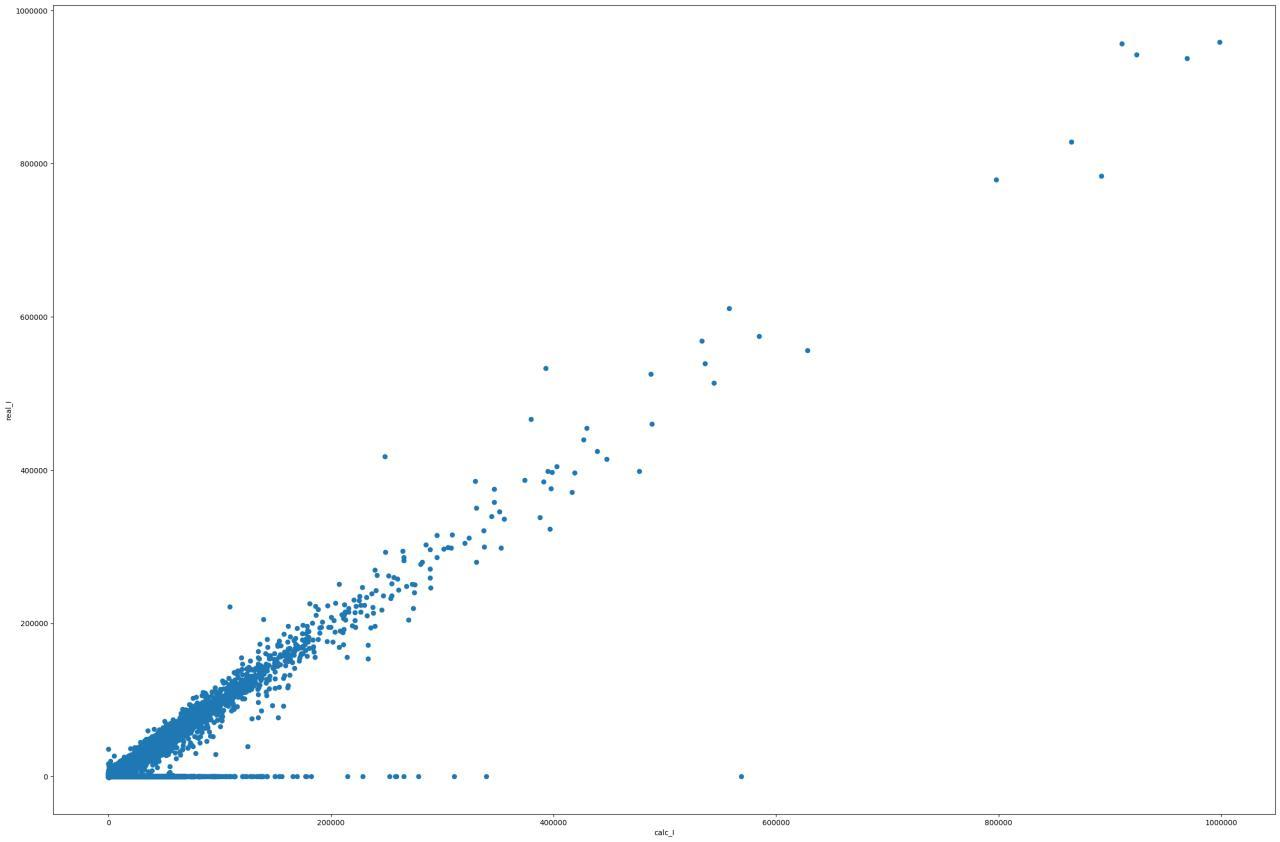
\includegraphics[width=\linewidth]{imgs/dist_lr.jpg}
  \caption{Нормализация с помощью линейной регрессии}\label{img:dist_lr}
\end{figure}


Рассчетные данные были получены из базы данных CCDC также в виде cif-файлов, обработаны идентично экспериментальным и отправлены на суперкомпьютер. Размер датасета составил 150 000 фалов, по 4630 отражений в каждом. Нормализация данных проводилась на максимальное значение интенсивности из присутствовавших в файле отражений. Отрицательной стороной использования данных из CCDC вместо Acta Crystallographica E стало отсутствие в этих файлах тепловых факторов - параметров тепловх колебаний молекул, что снижает качество расчета структурных факторов, а значит и параметров отражений. Другая проблема с обучением на расчетных данных - отсутствие  

\subsection{Обучение на экспериментальных данных}
Полученные из Acta E и обработанные данные были отправлены на С/К <<Харизма>>, было запущено обучение простейшей модели(рис. \ref{img:model1}) - полносвязного перцетпрона из трех слоев, с размером слоя равным размеру входных и выходных данных.  

\begin{figure}[!h]

\includegraphics[width=\linewidth]{imgs/placeholder.jpeg}
\caption{Архитектура простой полносвязной нейросети}
\label{img:model1}
\end{figure}

Результат обучения отрицательный - модель очень сильно переобучается, демонстрируя хорошие показатели на обучающих данных и очень плохие - на тестовом.Этот эффект наблюдается как на графике(рис. \ref{fig:acc_7k}) точности от эпохи обучения, так и на графике (рис. \ref{fig:loss_7k}) функции потерь от эпохи обучения.

\begin{figure}[!h]
\minipage{0.5\textwidth}
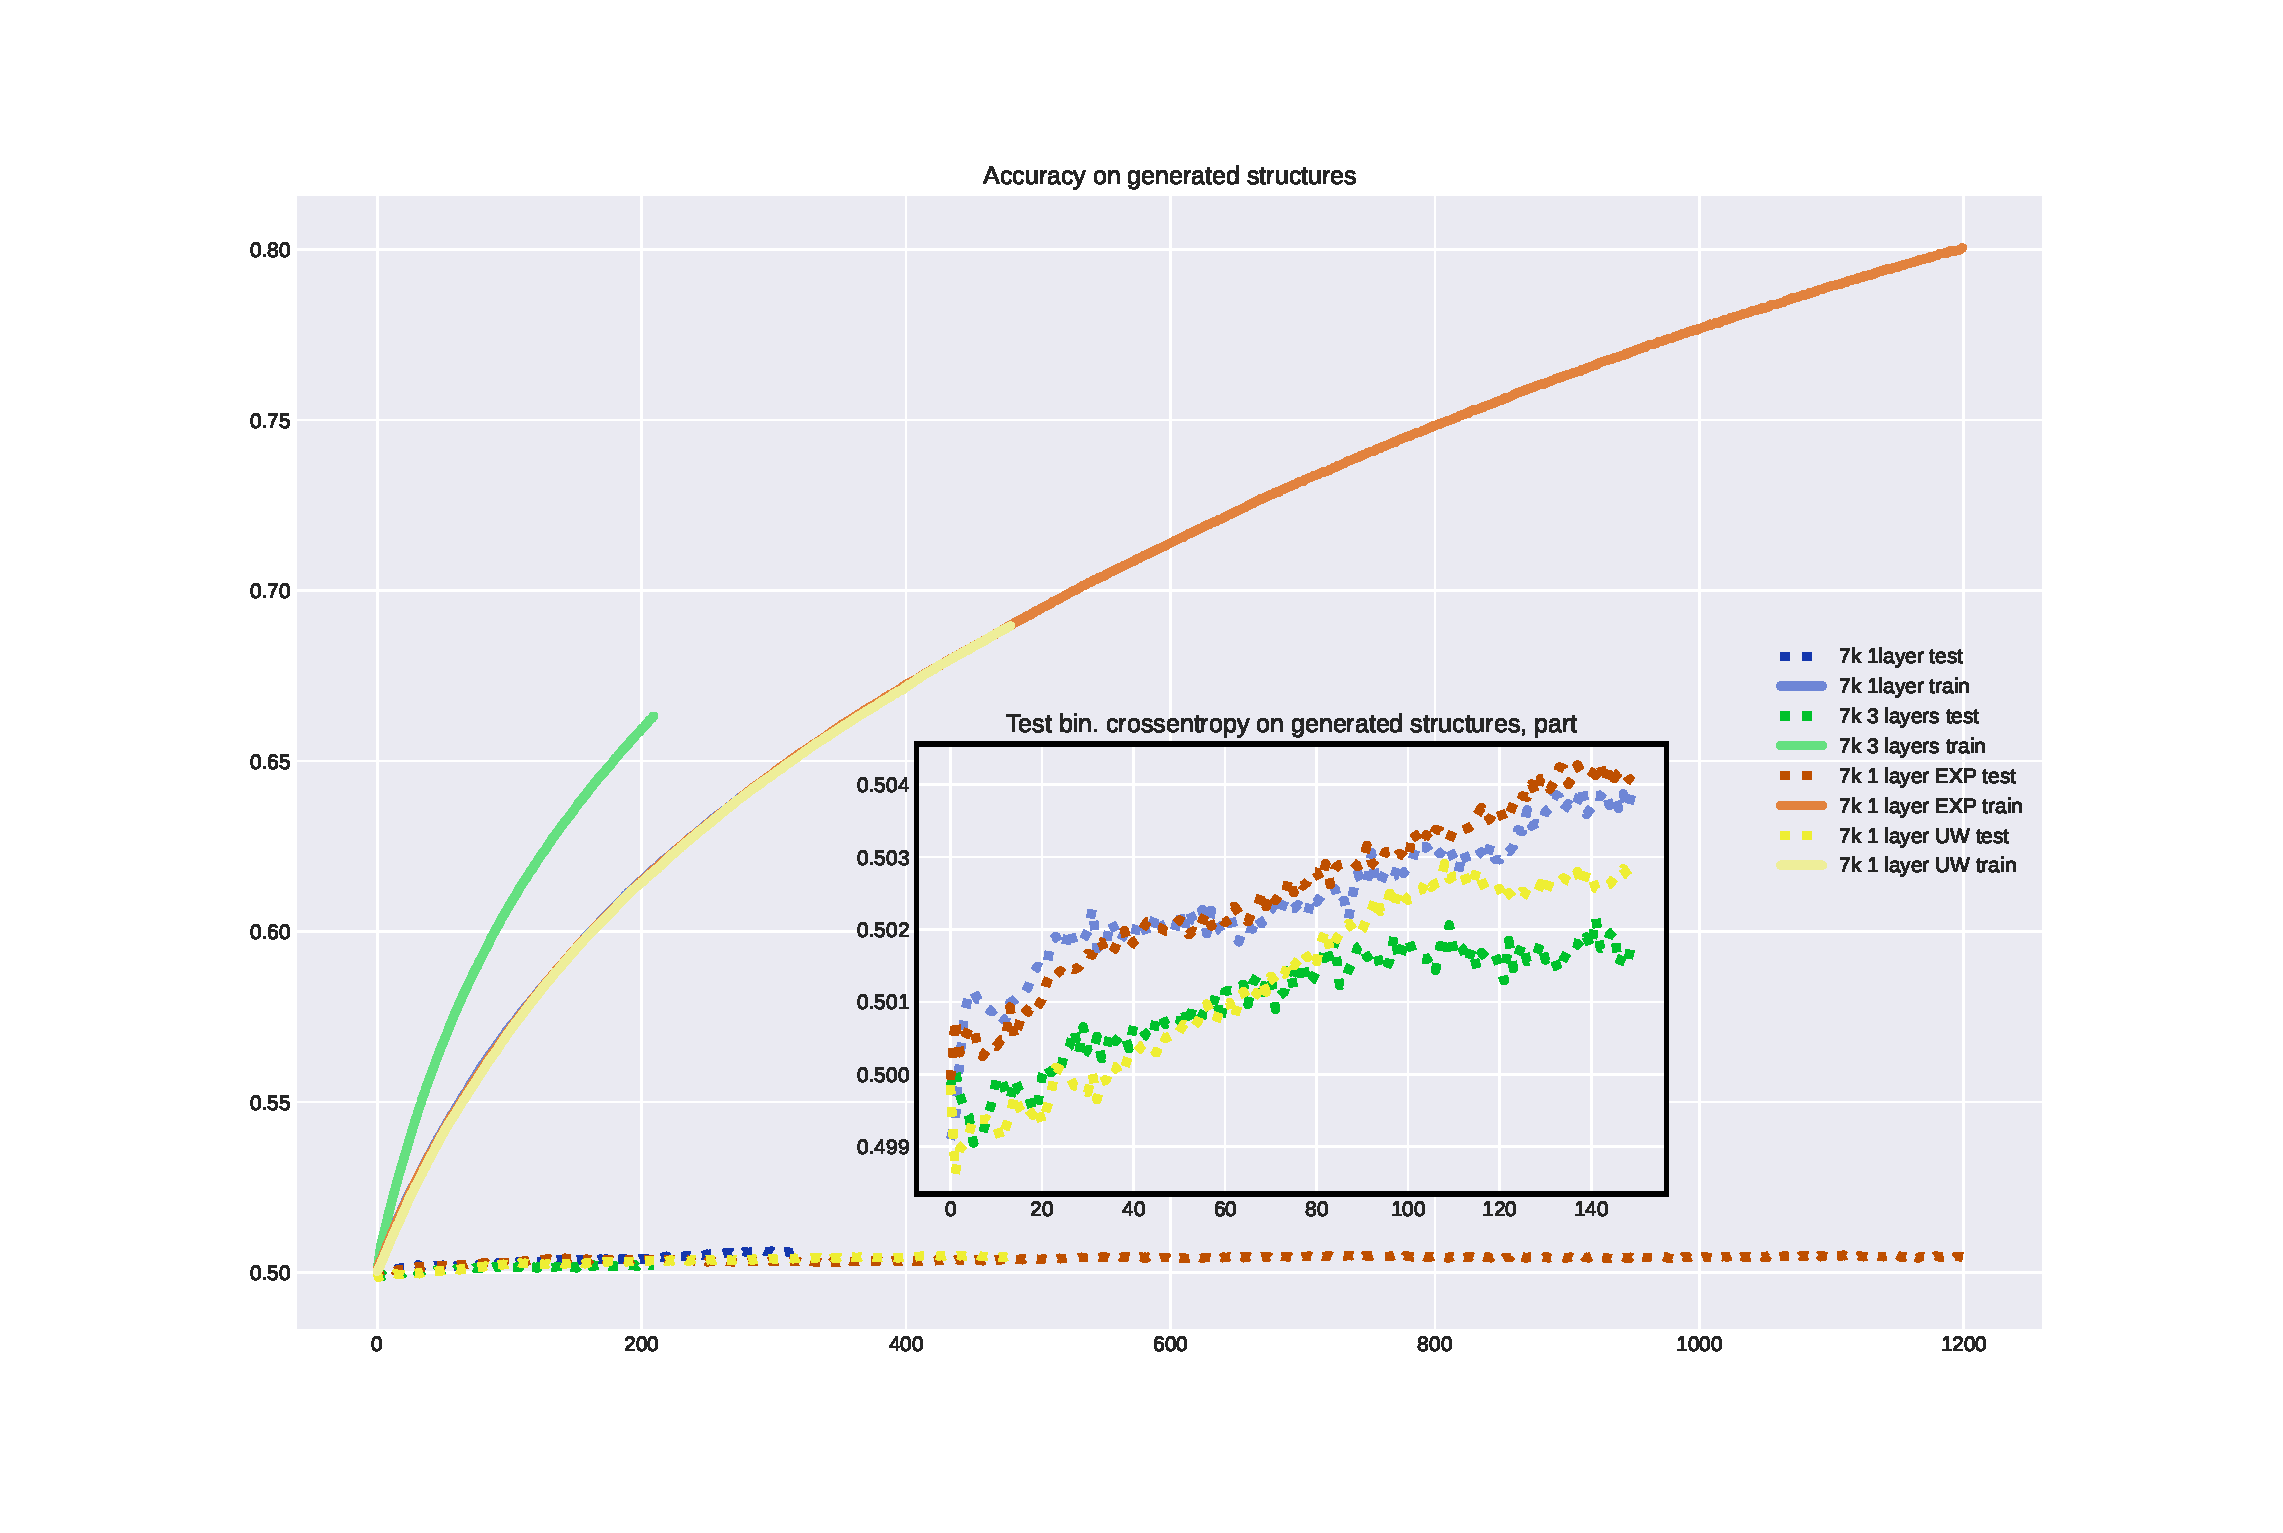
\includegraphics[width=\linewidth]{imgs/acc-7k.eps}
  \caption{Точность простой полносвязной нейросети в процессе обучения}\label{fig:acc_7k}
\endminipage\hfill
\minipage{0.5\textwidth}%
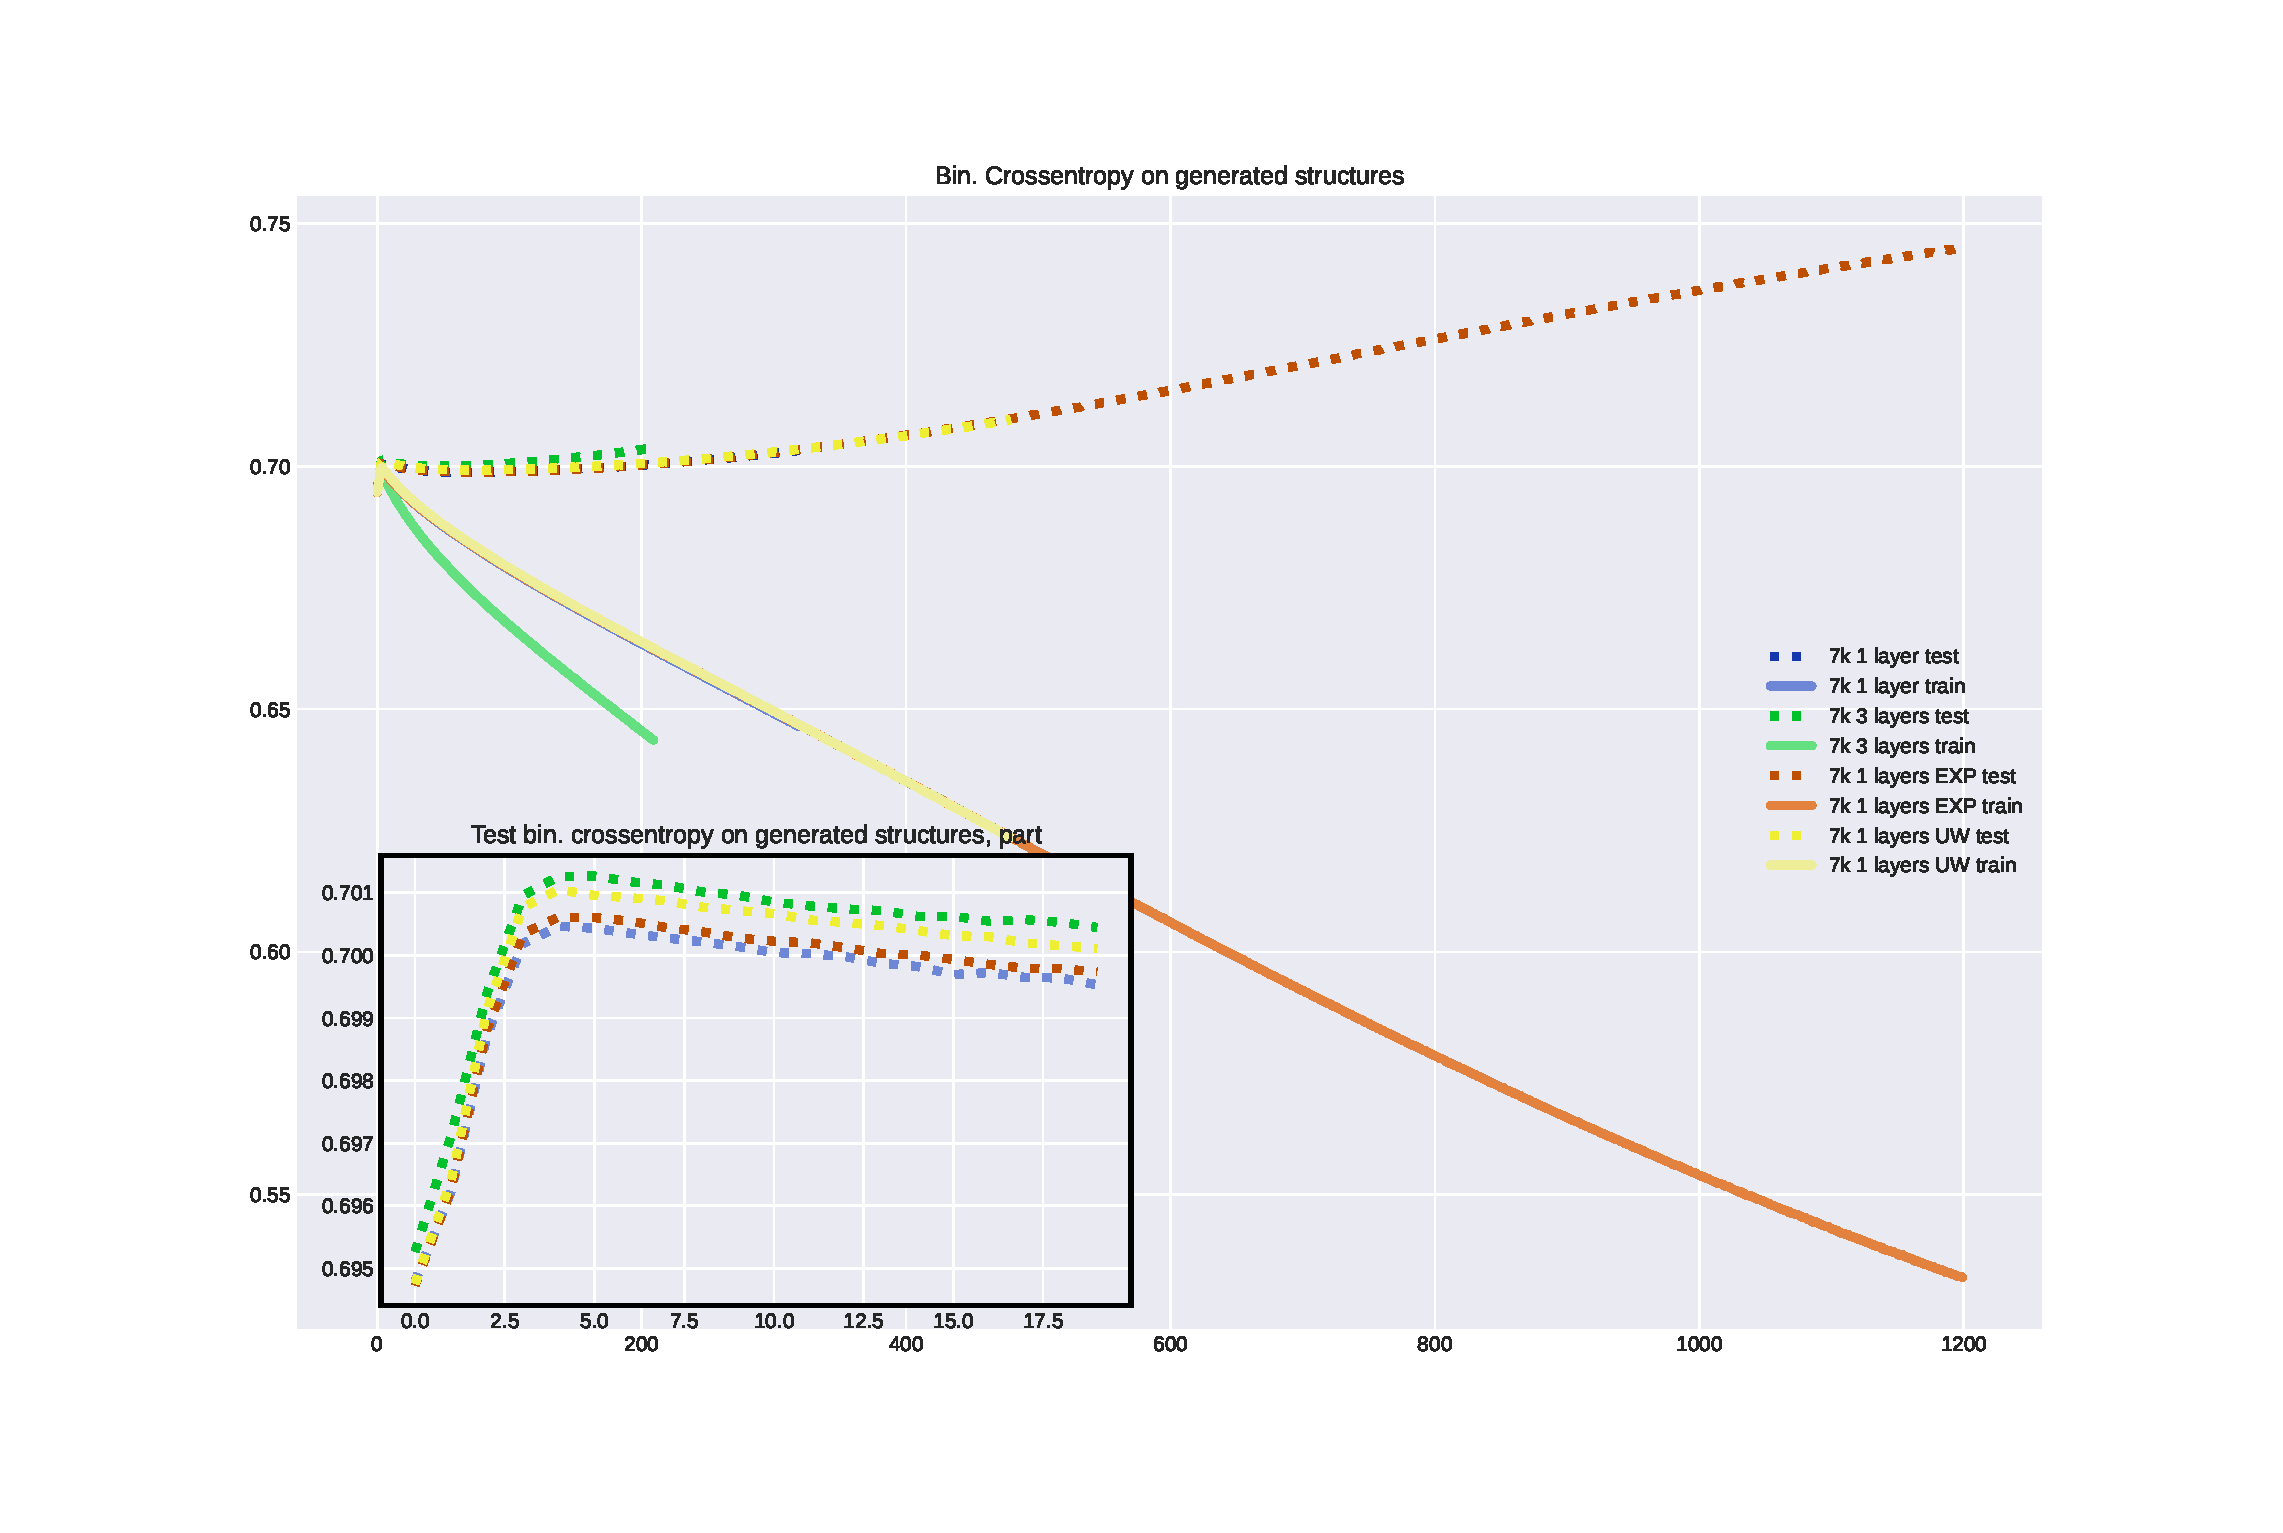
\includegraphics[width=\linewidth]{imgs/loss-7k.eps}
  \caption{Функция потерь простой полносвязной нейросети в процессе обучения}\label{fig:loss_7k}
\endminipage
\end{figure}

Из этого был сделан вывод о том, что данных для обучения модели недостаточно, и необходимо увеличить датасет. Другим возможным путем решения проблемы переобучения является снижение запоминающей способности сети путем добавления дропаутов, регуляризации, снижения количества нейронов в скрытых слоях сети и числа скрытых слоев.

\subsection{Обучение нейронной сети на данных CCDC}

Было проведено обучение нейросети на данных CCDC с разными гиперпараметрами и размером датасета. Для ускорения расчетов в части экспериментов были отброшены отражения с наибольшими индексами $h,k,l$, оставлены лишь удовлетворяющие условию $h^2+k^2+l^2<50$. После отбрасывания в каждом файле осталось по 709 отражений. Получены следующие результаты:

Для части датасета в 50 тысяч файлов, с отброшенными дальними отражениями была проведена проверка относительного качества обучения двух моделей: с одним внутренним слоем из 709 нейронов и с тремя внутренними слоями из 709 нейронов. Графики обучения (рис. \ref{fig:acc_50k}, \ref{fig:loss_50k}) демонстрируют сильное переобучение в обоих случаях, однако в случае с одним слоем оно менее выражено. Это говорит о том, что обе модели имеют избыточную запоминающую способность.

\begin{figure}[!h]
\minipage{0.5\textwidth}
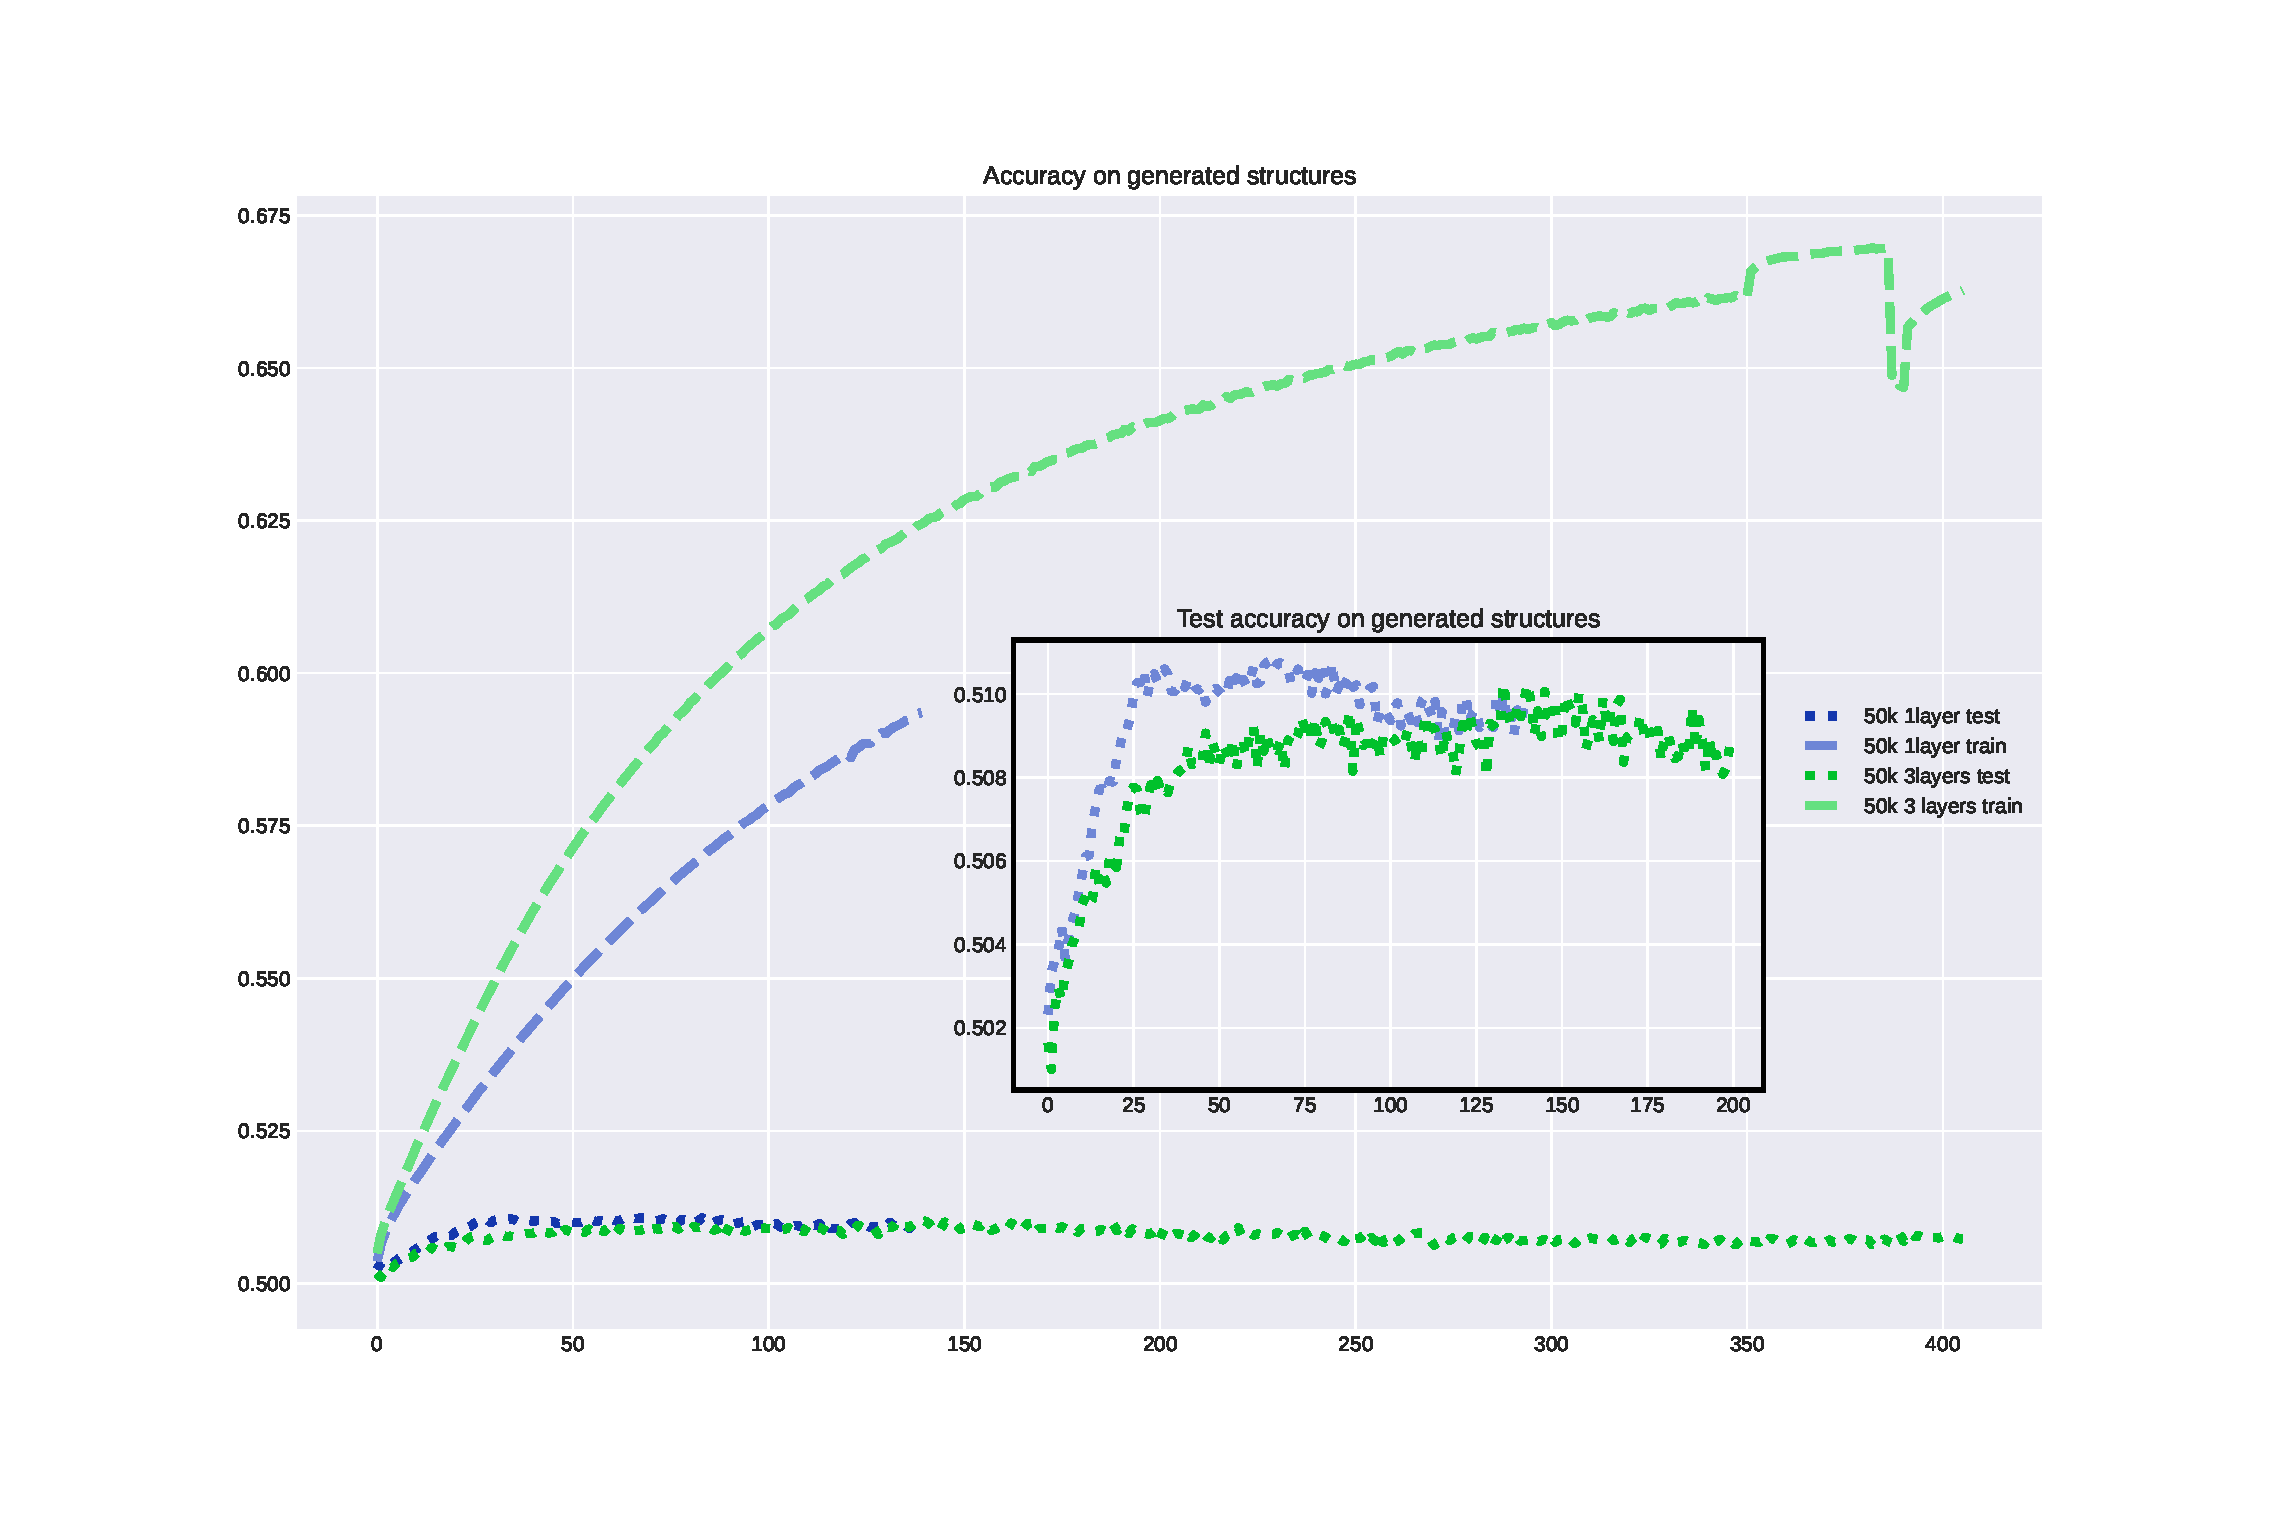
\includegraphics[width=\linewidth]{imgs/acc-50k.eps}
  \caption{Точность нейросети с одним и тремя слоями}\label{fig:acc_50k}
\endminipage\hfill
\minipage{0.5\textwidth}%
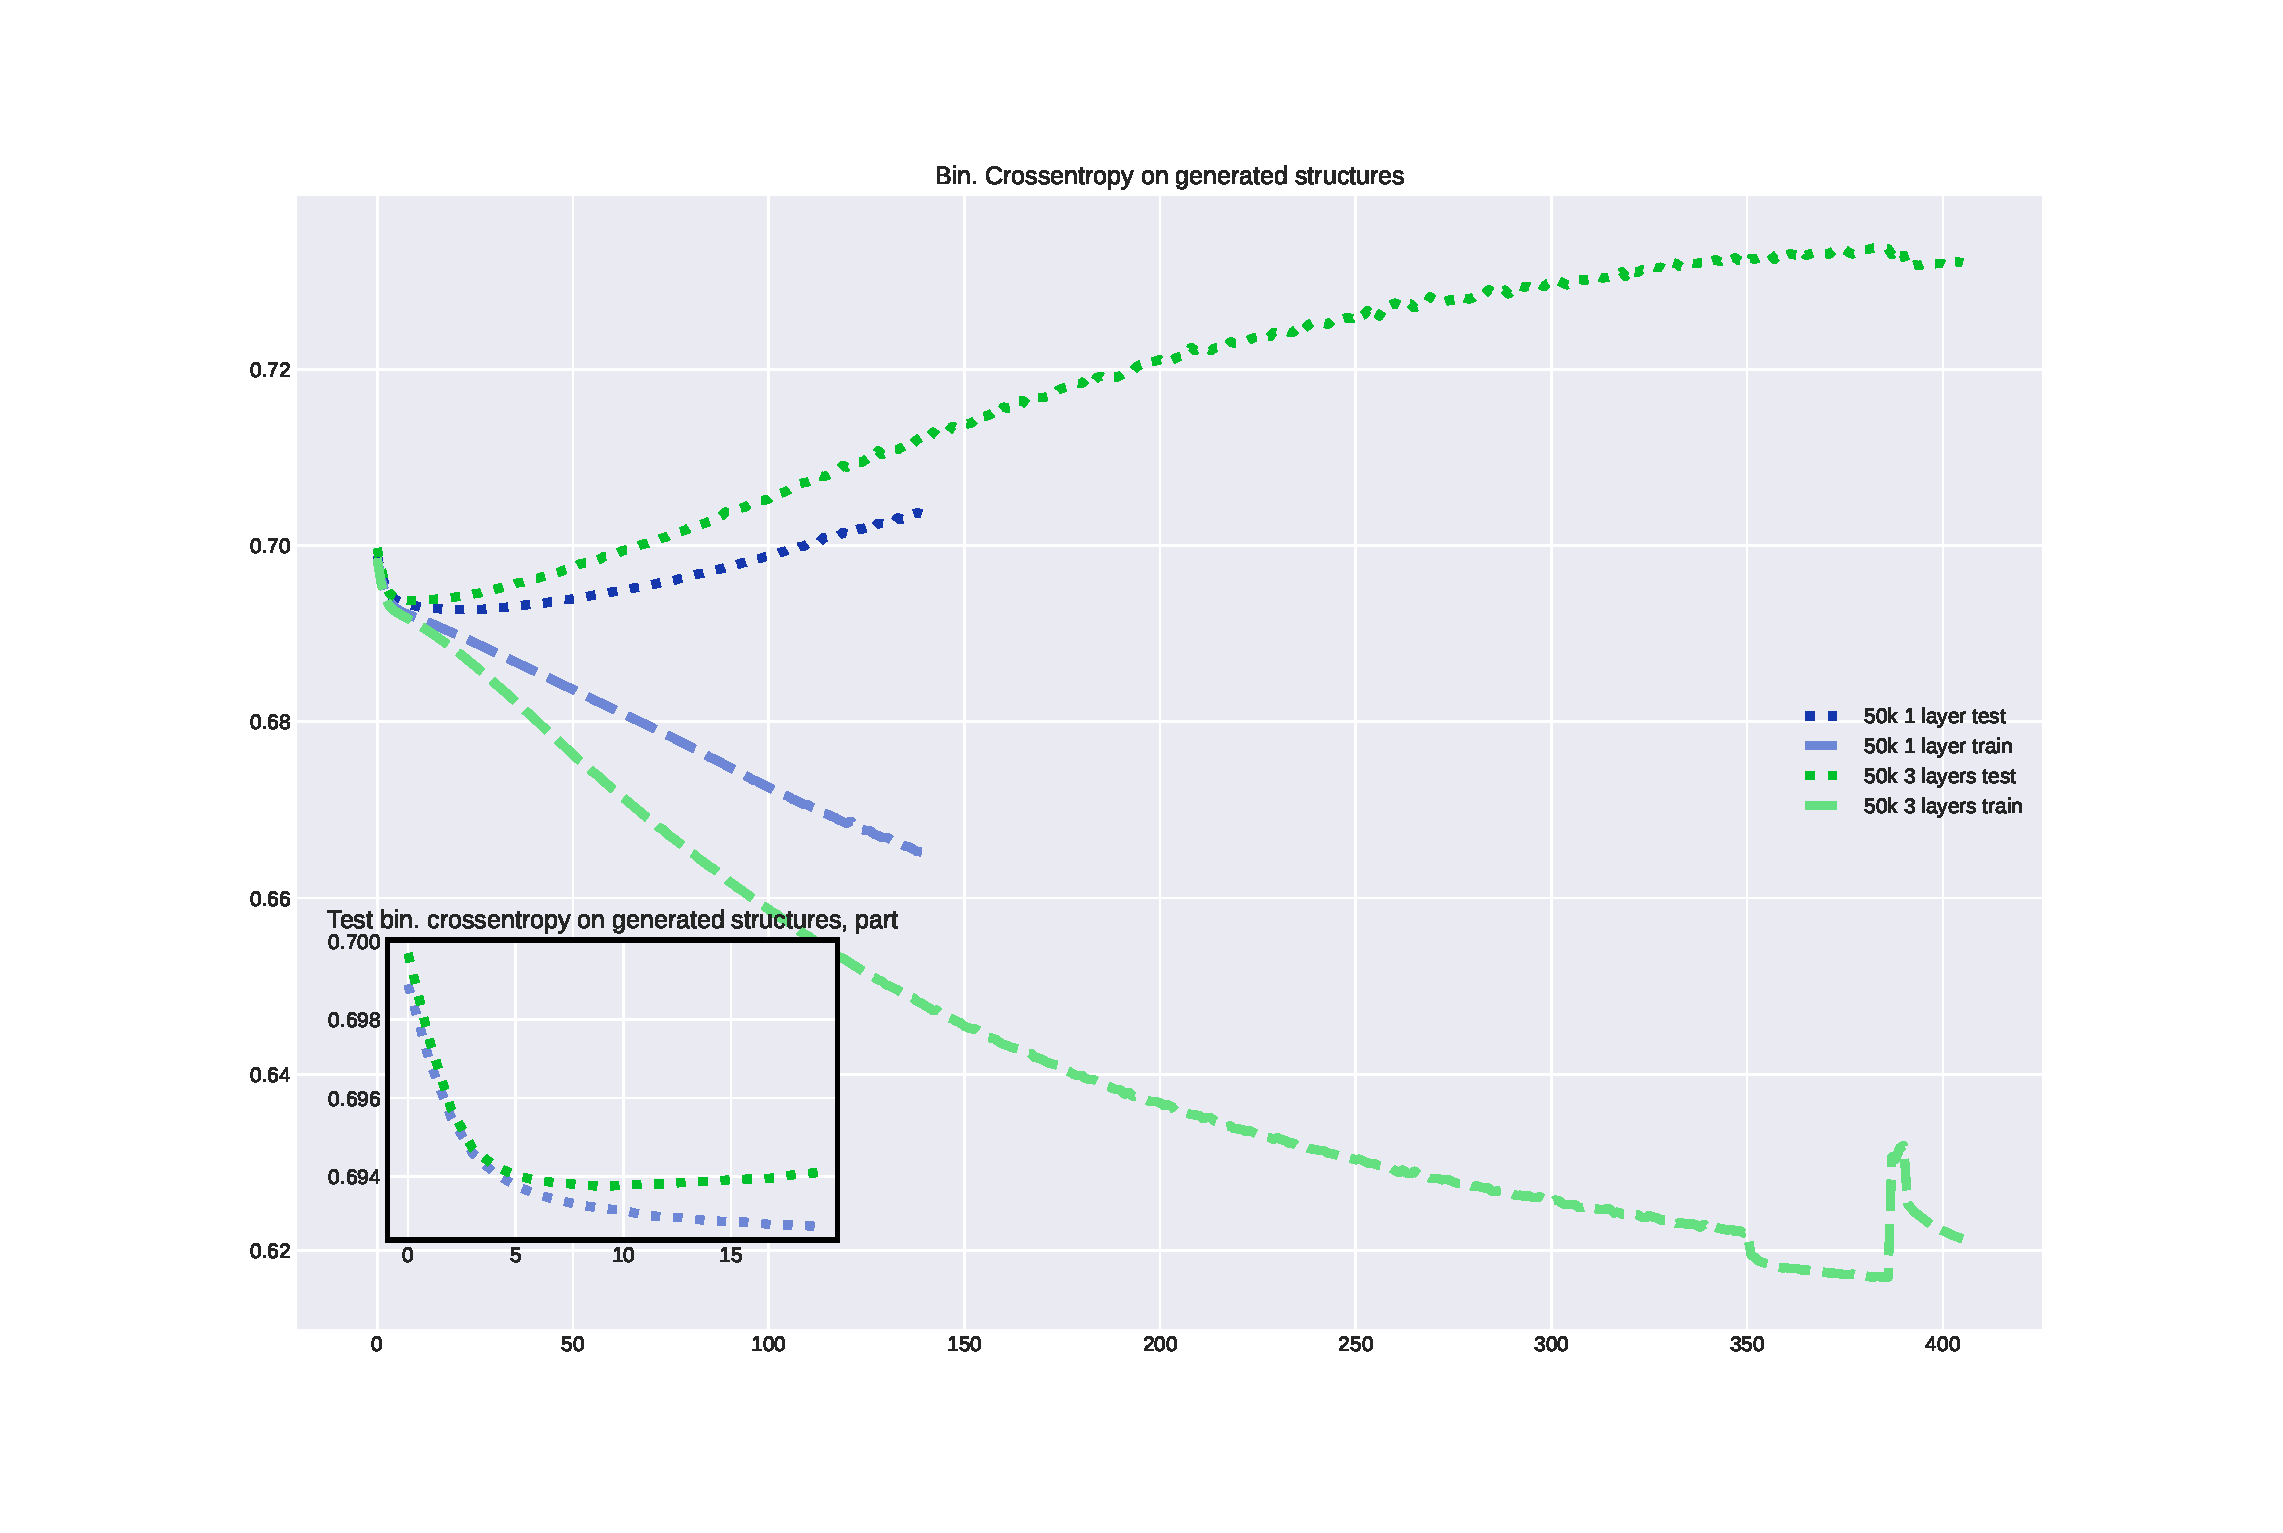
\includegraphics[width=\linewidth]{imgs/loss-50k.eps}
  \caption{Функция ошибки нейросети с одним и тремя слоями}\label{fig:loss_50k}
\endminipage
\end{figure}

Был проверена зависимость качества обучения от размера датасета. Было проведено обучение на разном количестве данных - 7000 файлов, 50 тысяч файлов, 150 тысяч файлов, с отбросом дальних отражений. На графиках обучения(рис. \ref{fig:acc_1l_ndata}, \ref{fig:loss_1l_ndata}) видно что больший размер датасета приводит к меньшему переобучению, %ну вот кто бы мог подумать?..

\begin{figure}[!h]
\minipage{0.5\textwidth}
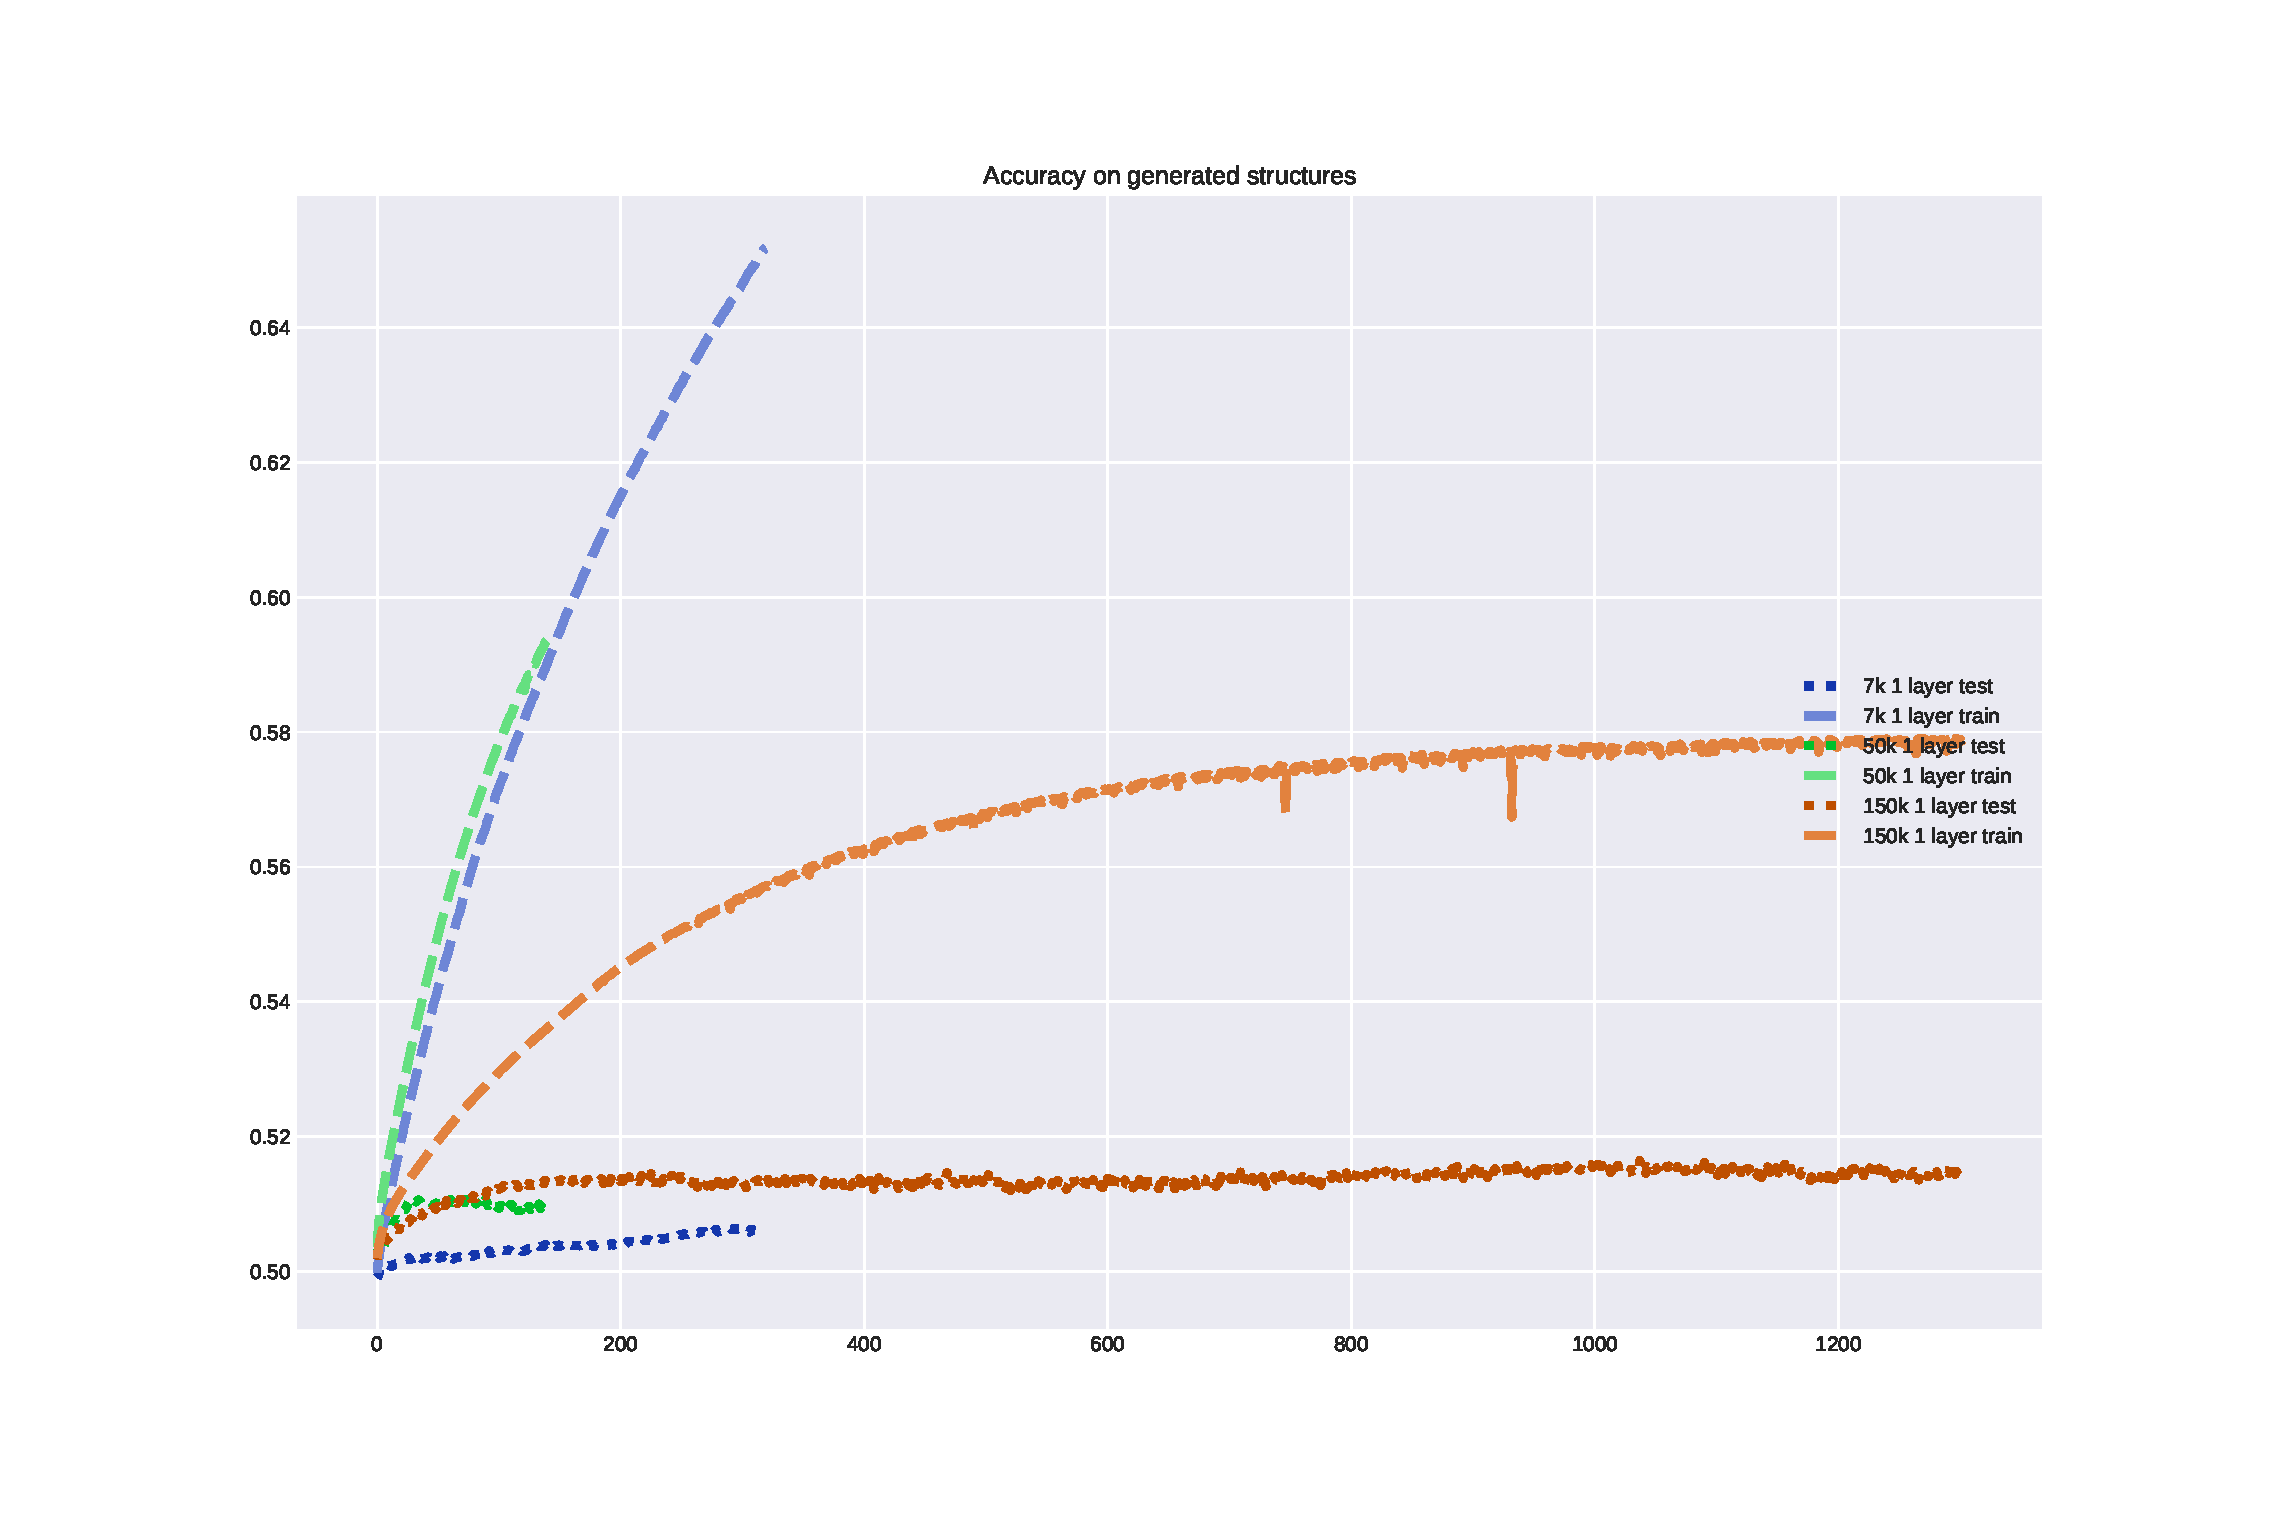
\includegraphics[width=\linewidth]{imgs/acc-1l_ndata.eps}
  \caption{Точность нейросети с одним слоем на разном количестве данных}\label{fig:acc_1l_ndata}
\endminipage\hfill
\minipage{0.5\textwidth}%
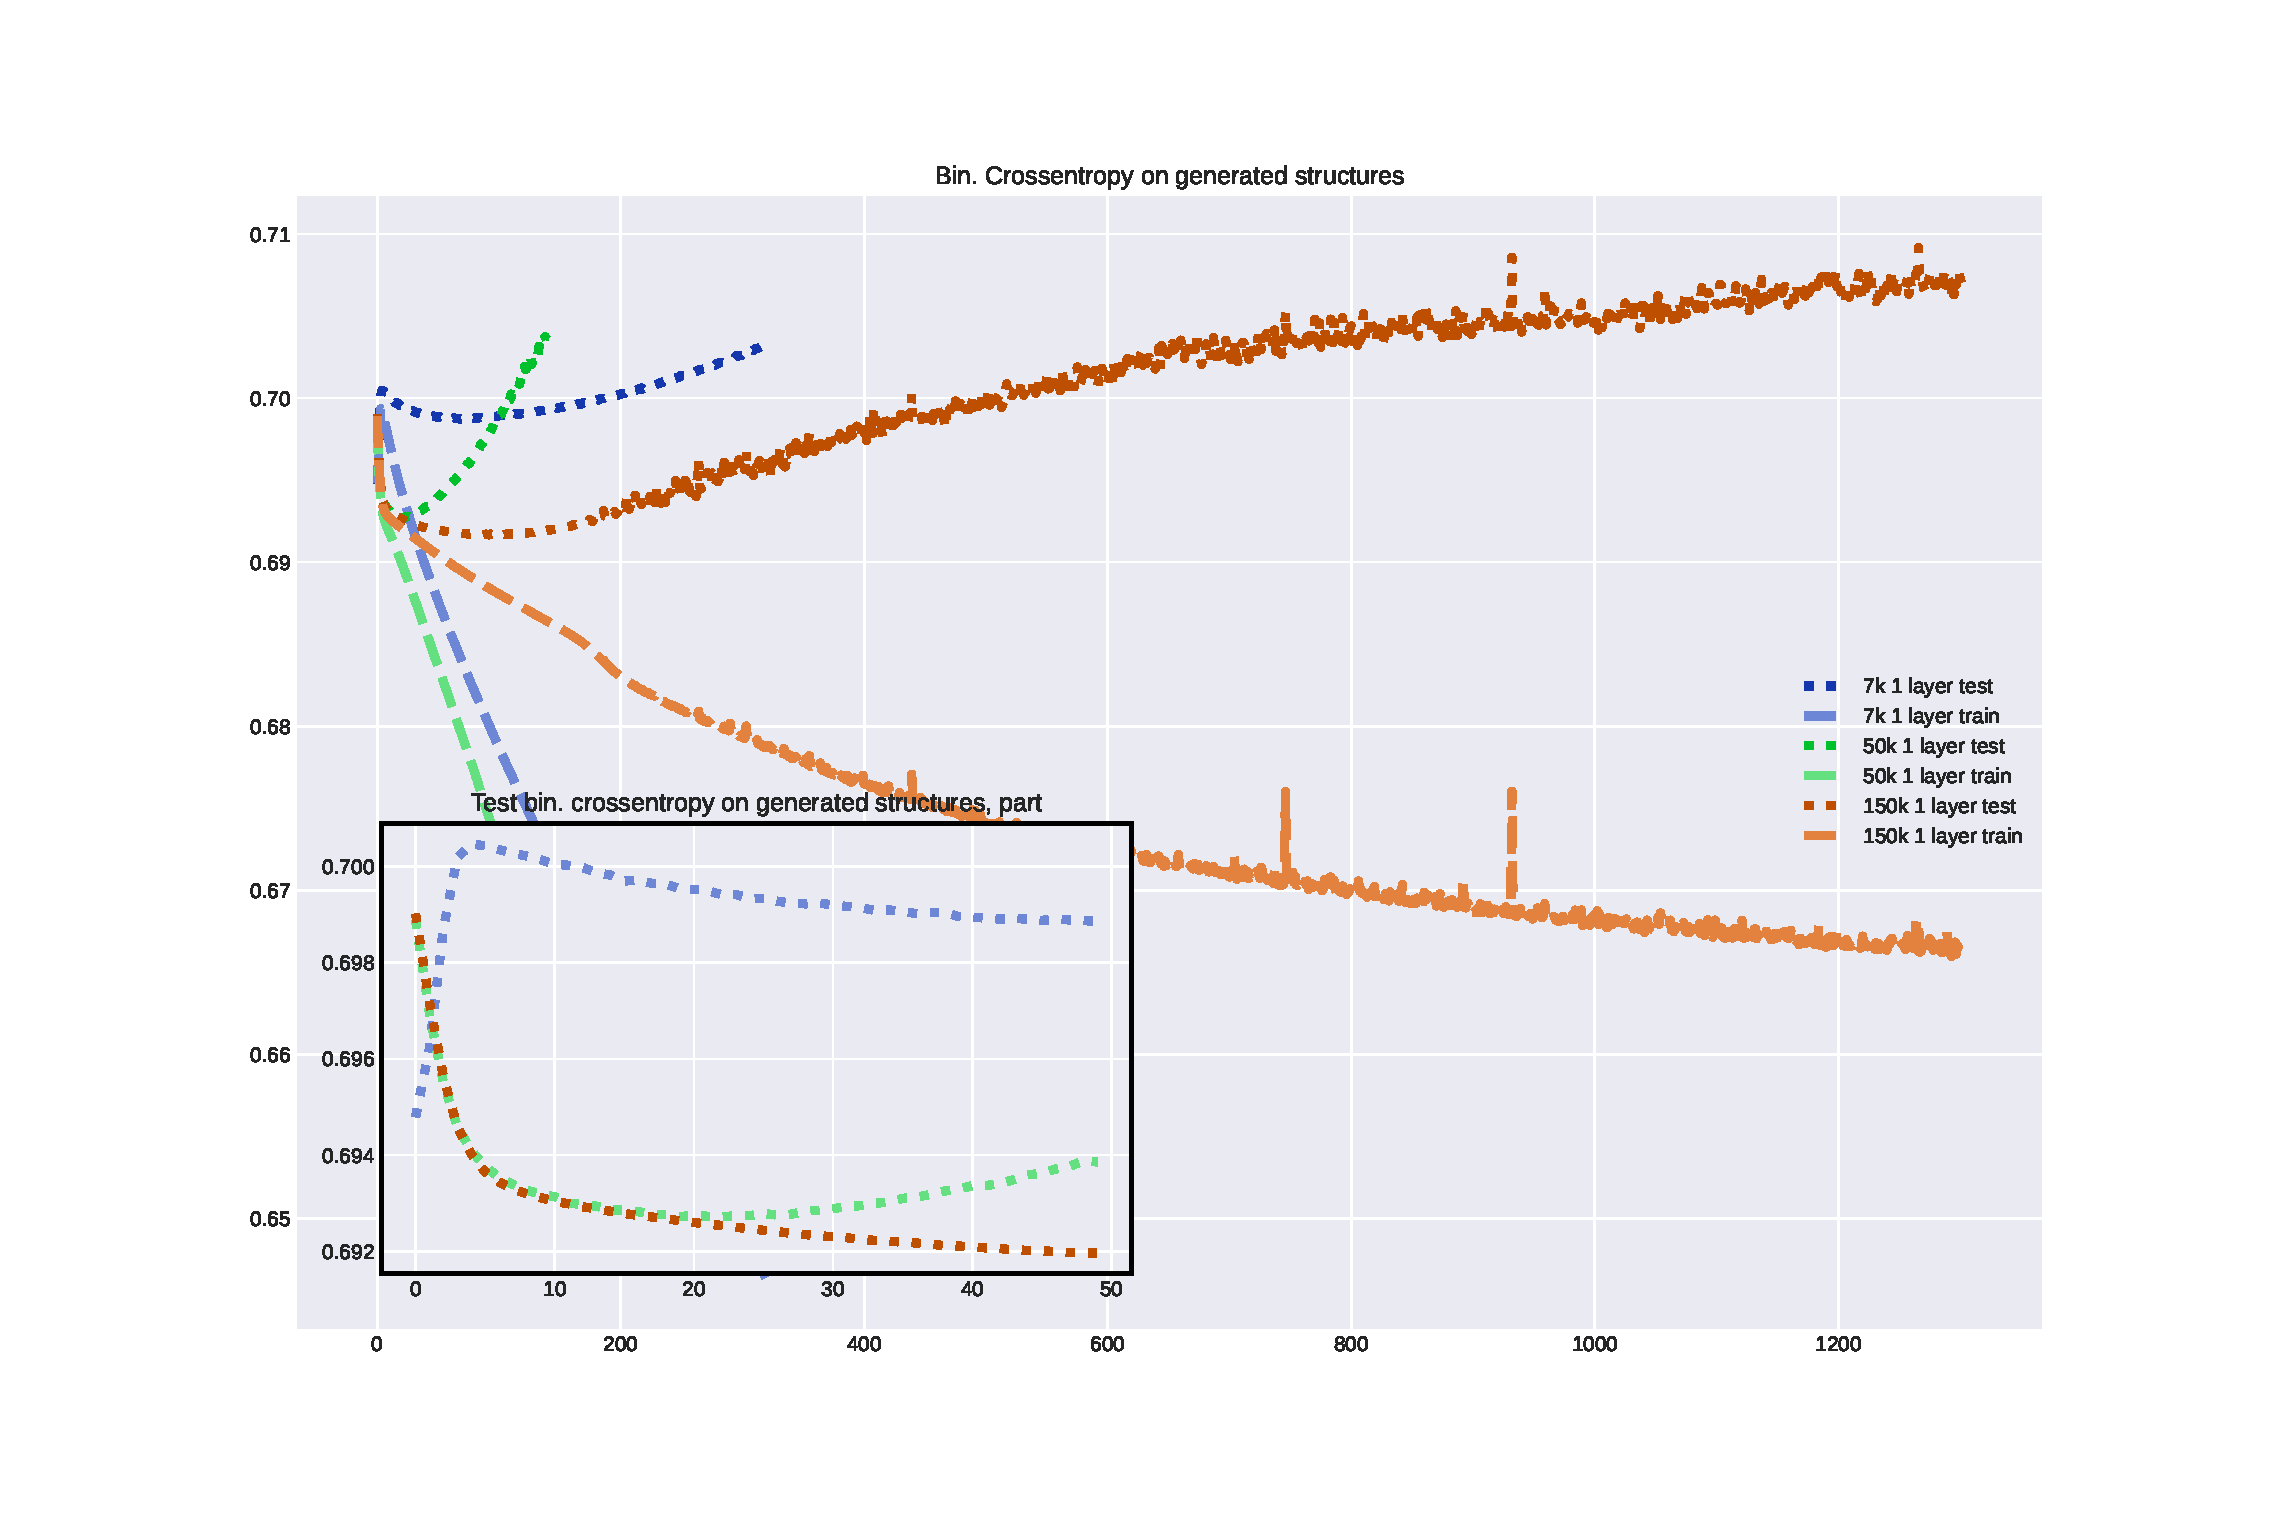
\includegraphics[width=\linewidth]{imgs/loss-1l_ndata.eps}
  \caption{Функция ошибки нейросети с одним слоем на разном количестве данных}\label{fig:loss_1l_ndata}
\endminipage
\end{figure}


Тот же результат был получен и при обучении нейросети из 3 слоев. Также было проведено обучение на 7000, 50 тысячах и 150 тысячах фалов. Заметно переобучение, оно уменьшается при увеличении размеров датасета, что можно видеть по рисункам \ref{fig:acc_3l_ndata}, \ref{fig:loss_3l_ndata}.
\begin{figure}[!h]
\minipage{0.5\textwidth}
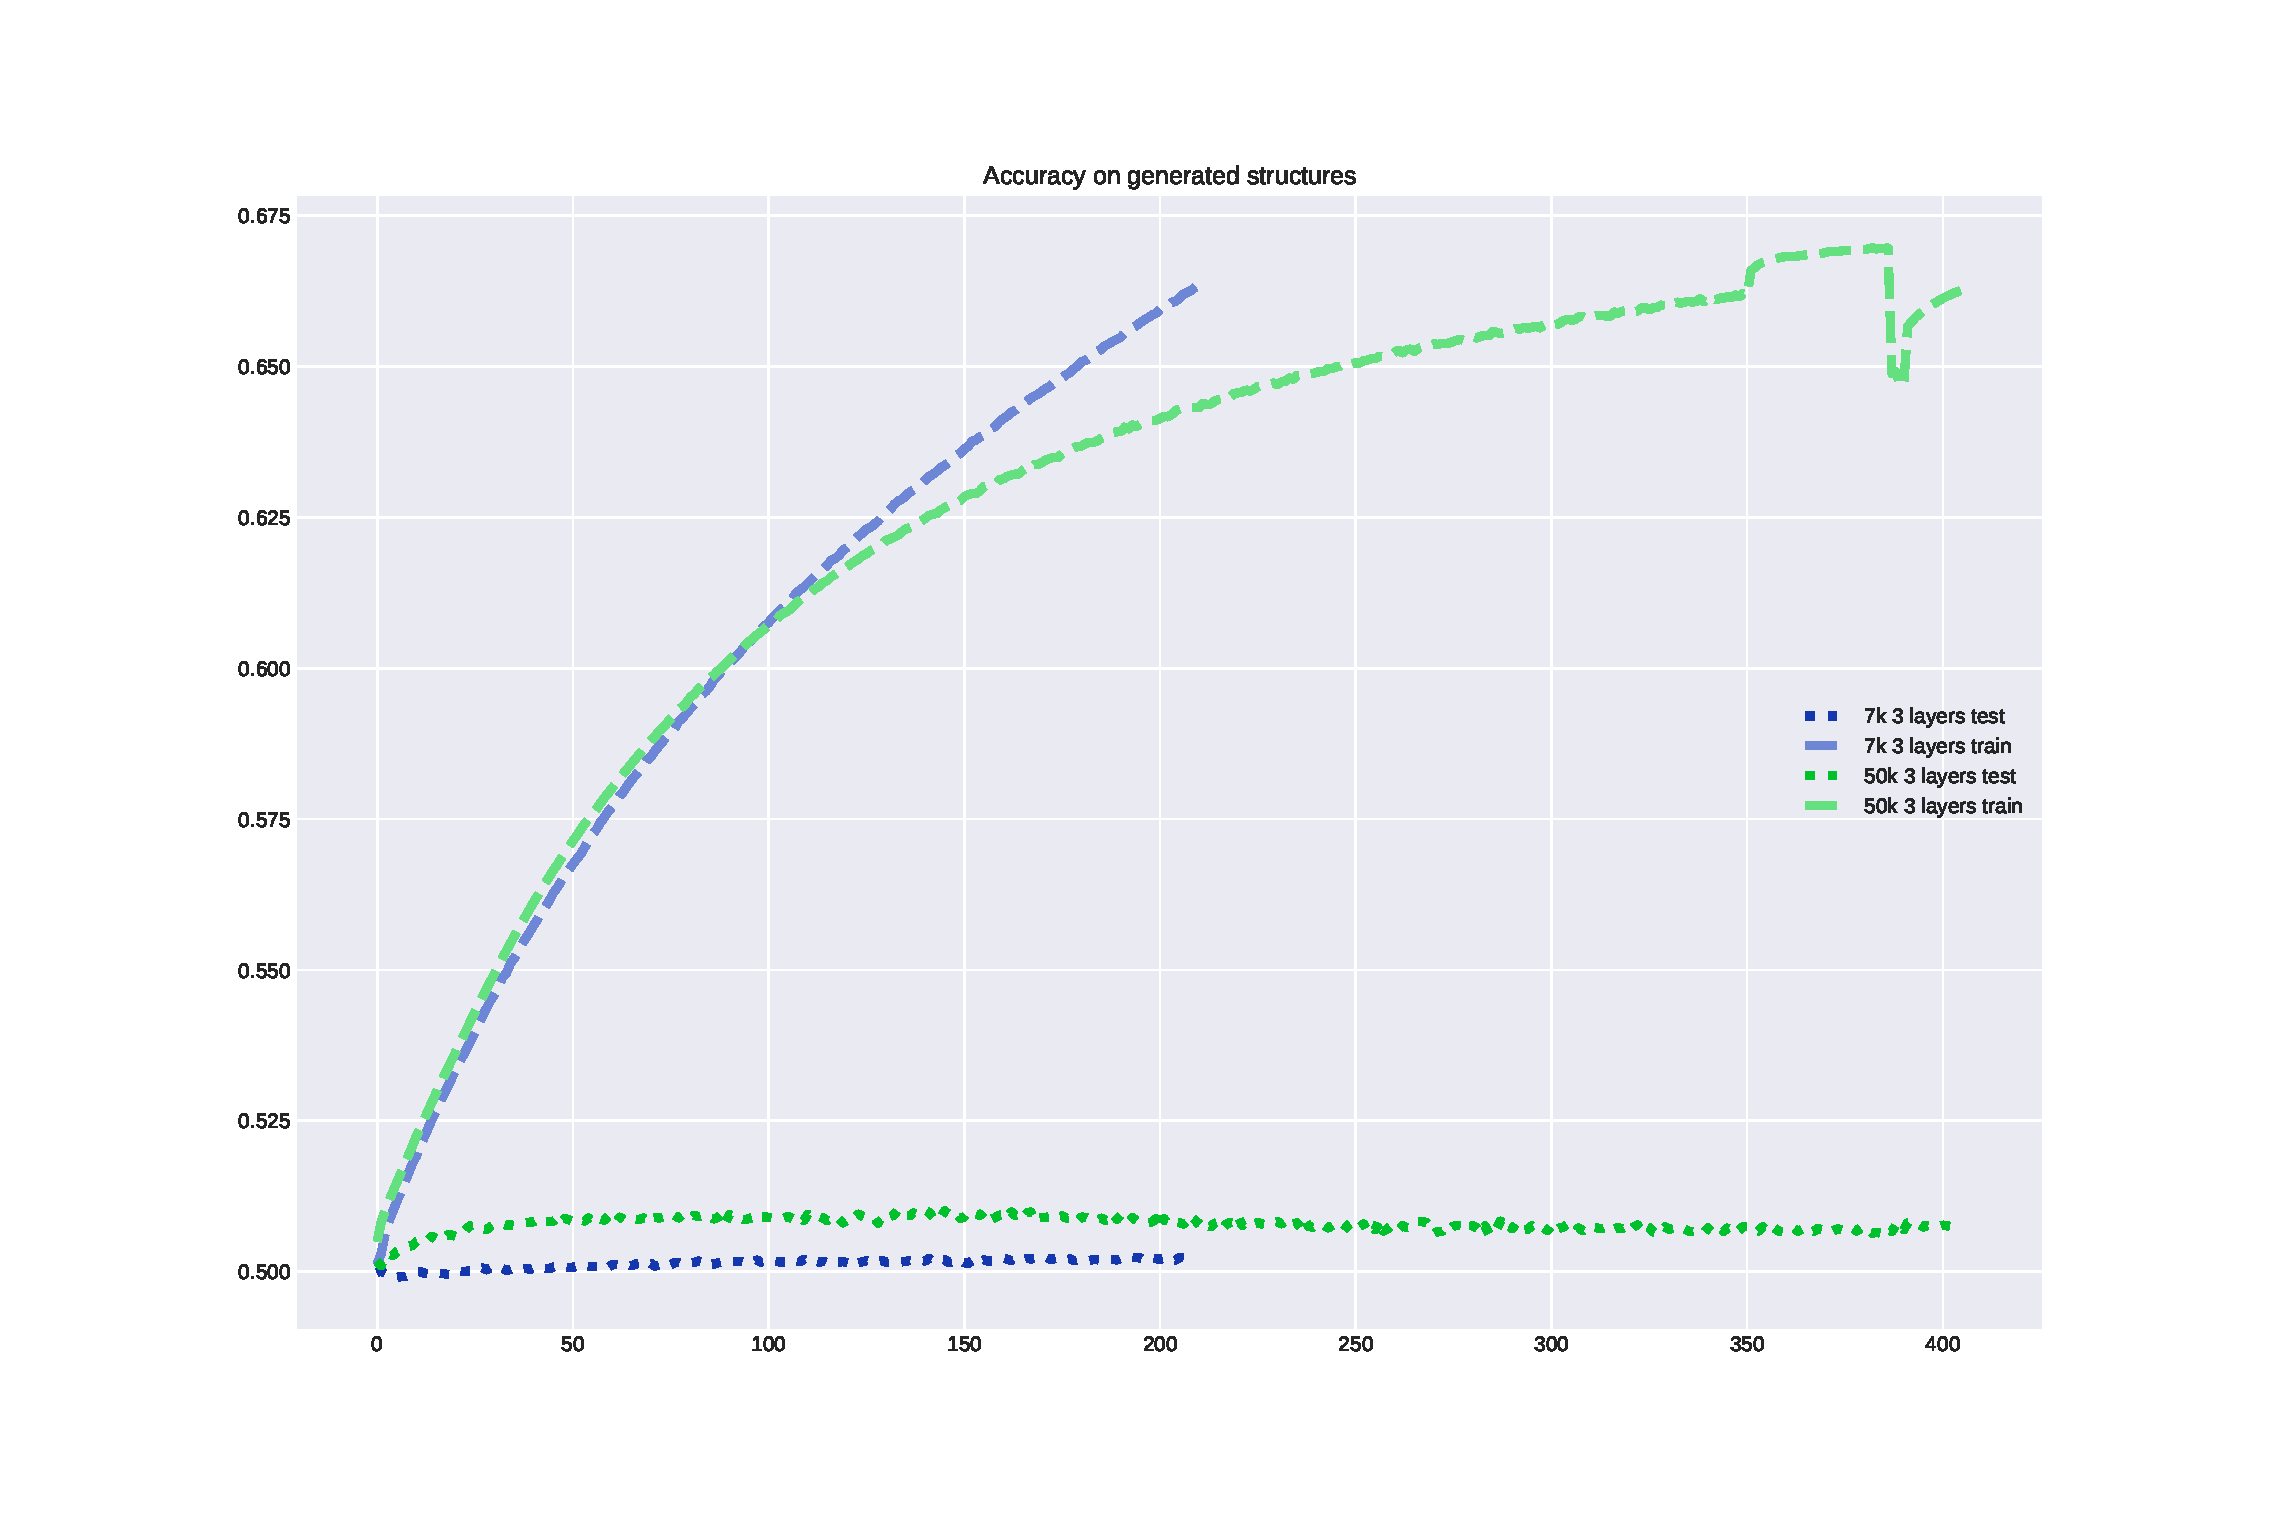
\includegraphics[width=\linewidth]{imgs/acc-3l_ndata.eps}
  \caption{Точность нейросети с одним слоем на разном количестве данных}\label{fig:acc_3l_ndata}
\endminipage\hfill
\minipage{0.5\textwidth}%
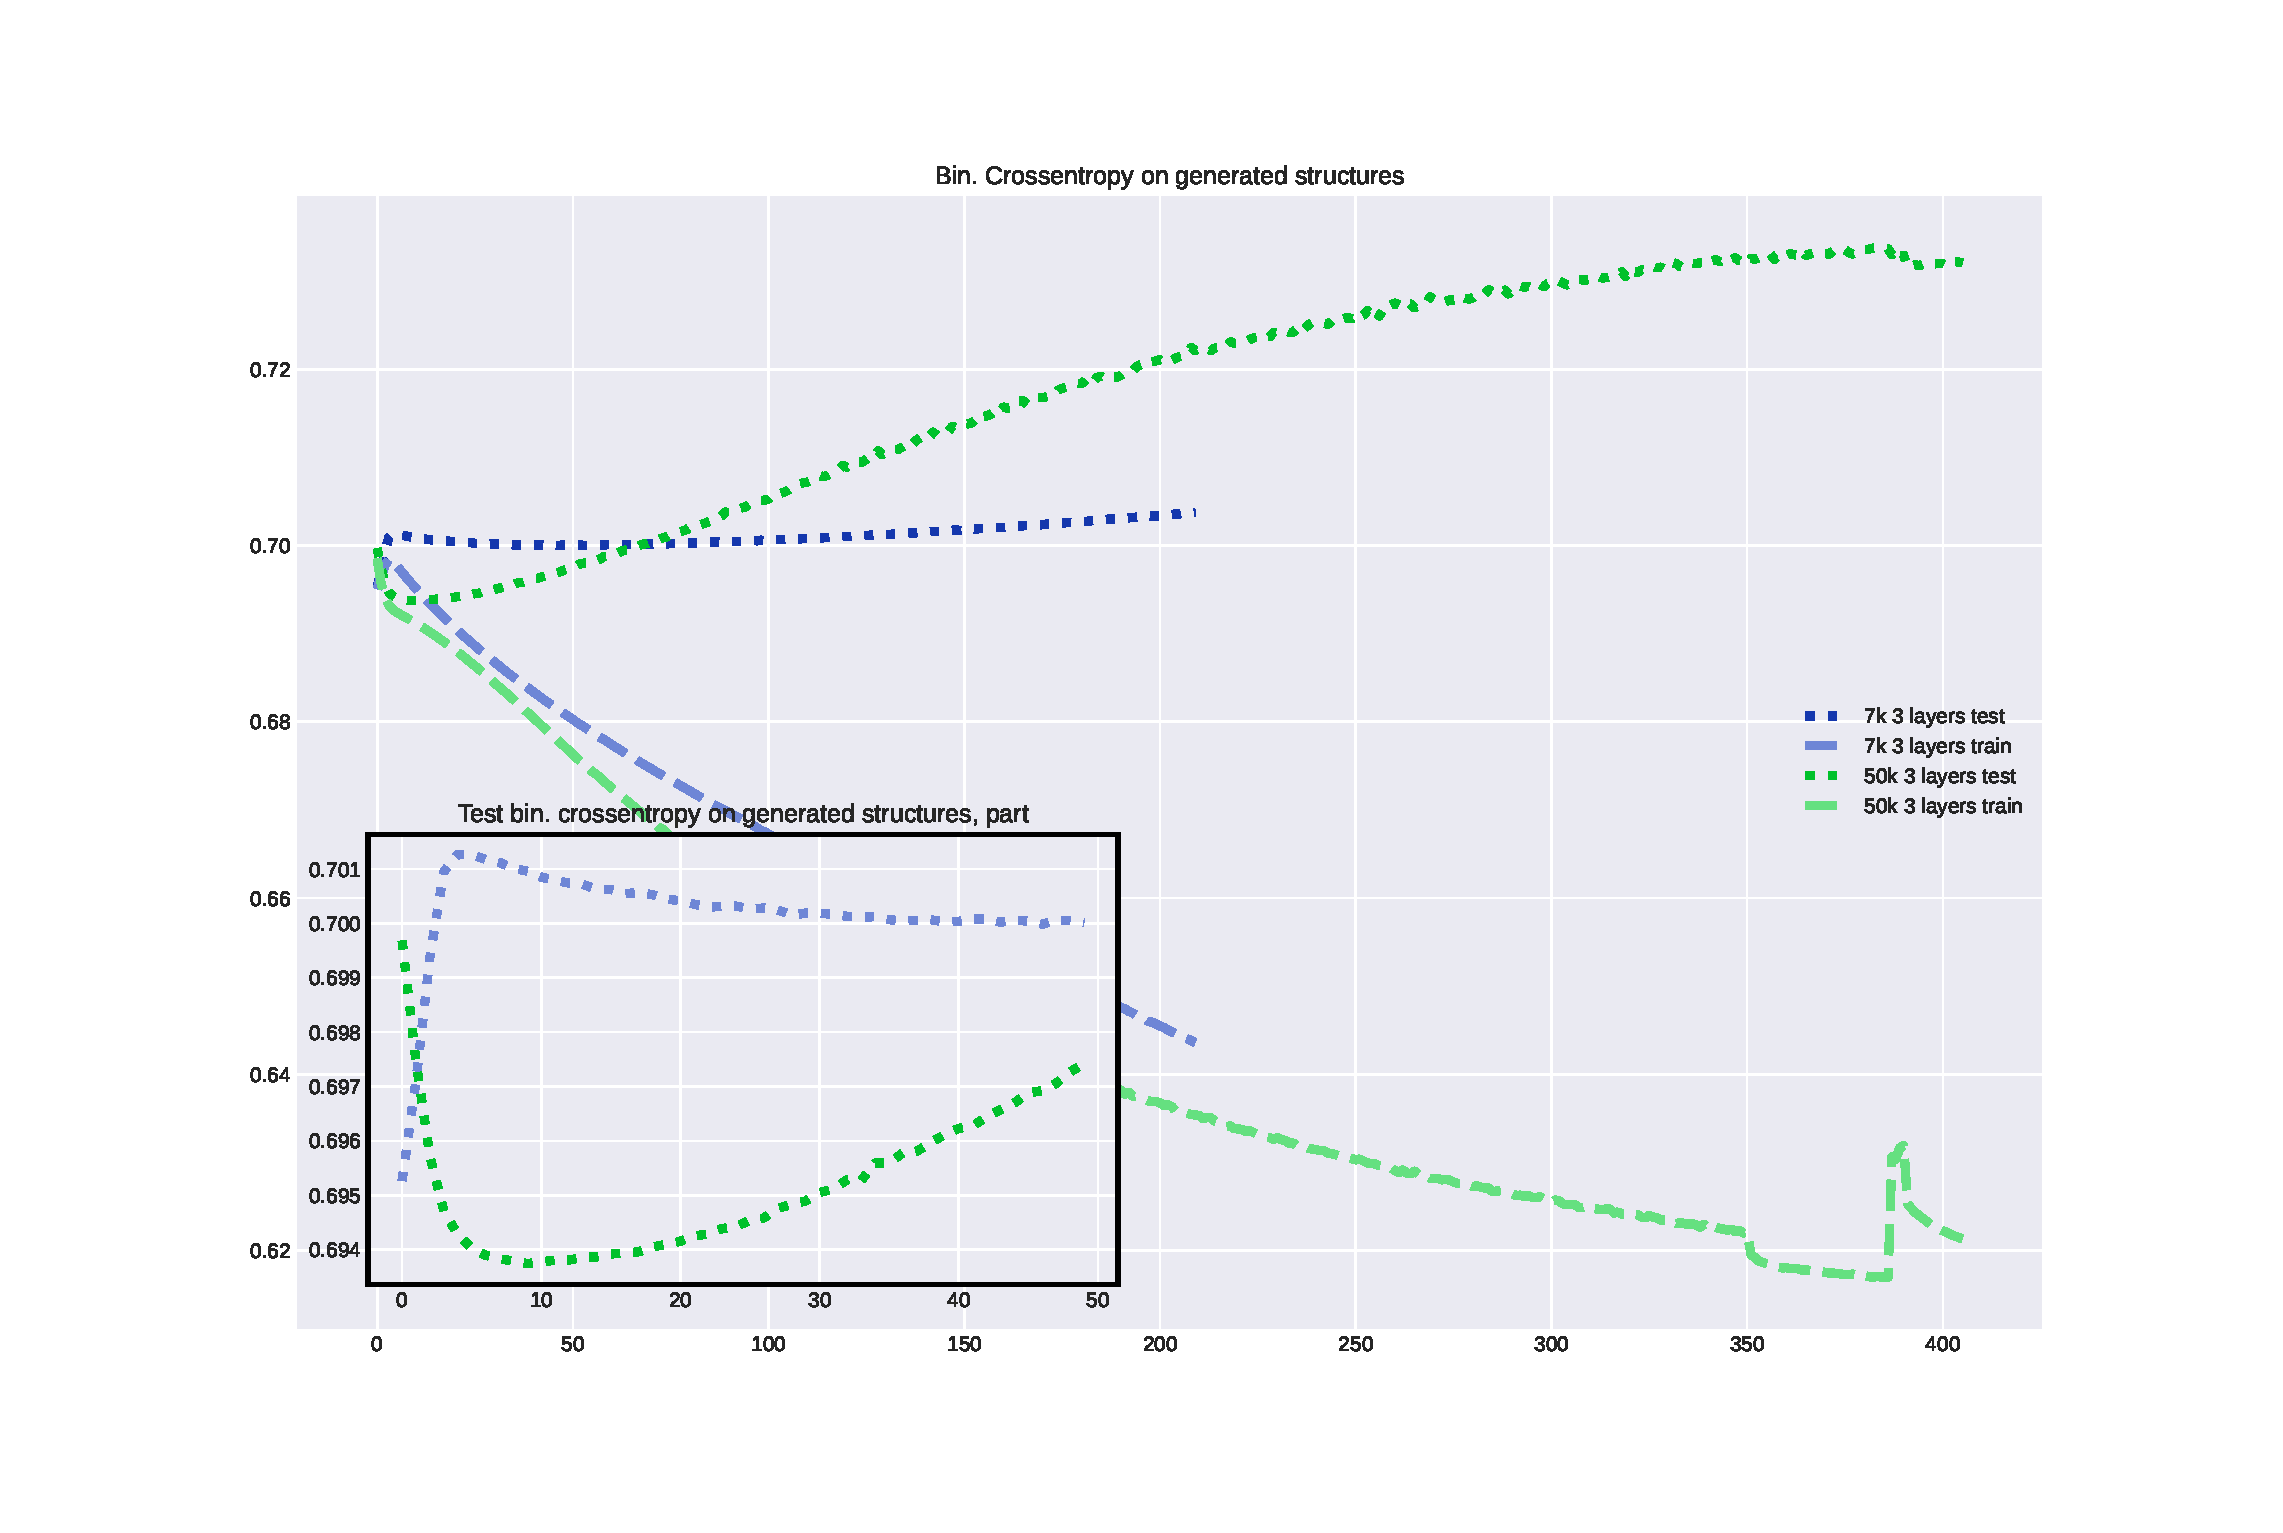
\includegraphics[width=\linewidth]{imgs/loss-3l_ndata.eps}
  \caption{Функция ошибки нейросети с одним слоем на разном количестве данных}\label{fig:loss_3l_ndata}
\endminipage
\end{figure}

\subsection{Зависимость качества обучения от типа весов}

Функцю ошибки, на основе которой проводится обучение модели, можно взвесить по какой-либо характеристике, как и метрику. Была исследована зависимость качества обучения от весов применемой в модели метрики. Результаты представлены на рис. \ref{fig:acc_weight}, \ref{fig:loss_weight}

Лучший результат дает обучнение с функцией ошибки взвешенной по интенсивности отражений. Взвешивание по экспоненте от интенсивности отражений, а также отсутствие взвешивания(равный вес всех отражений) дали незначительно худшие реультаты. 

\begin{figure}[!h]
\minipage{0.5\textwidth}
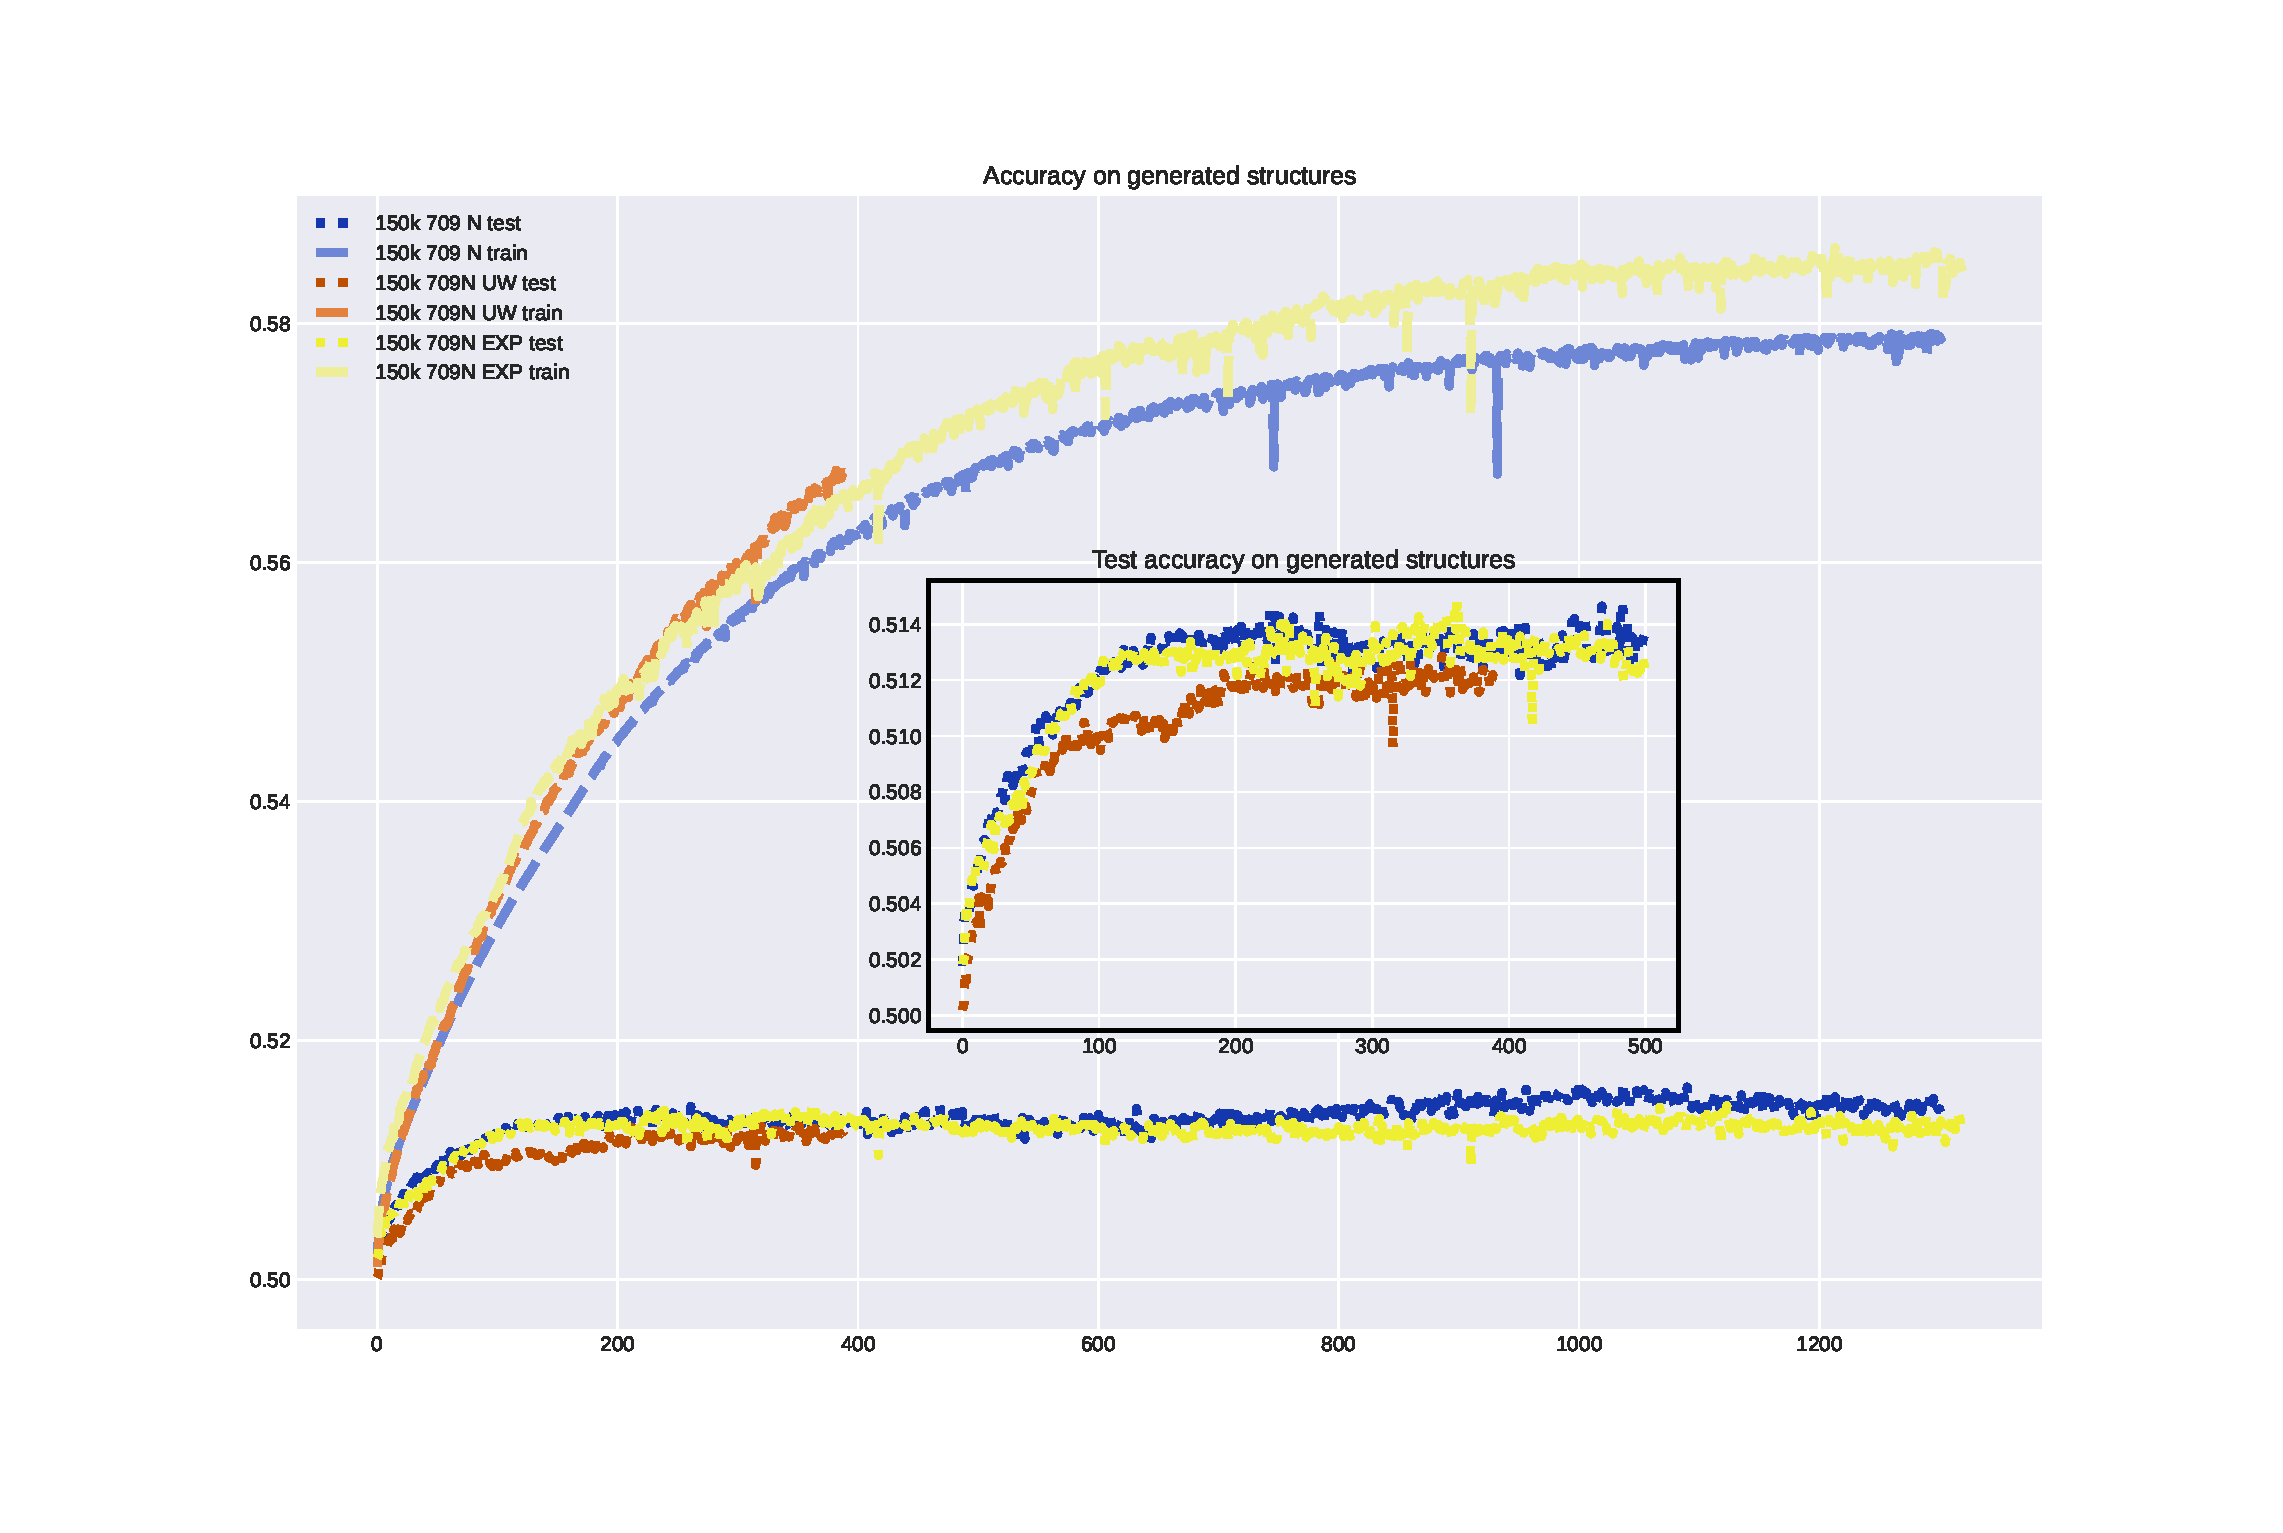
\includegraphics[width=\linewidth]{imgs/acc-weight.eps}
  \caption{Точность нейросети в зависимости от весов функции ошибки}\label{fig:acc_weight}
\endminipage\hfill
\minipage{0.5\textwidth}%
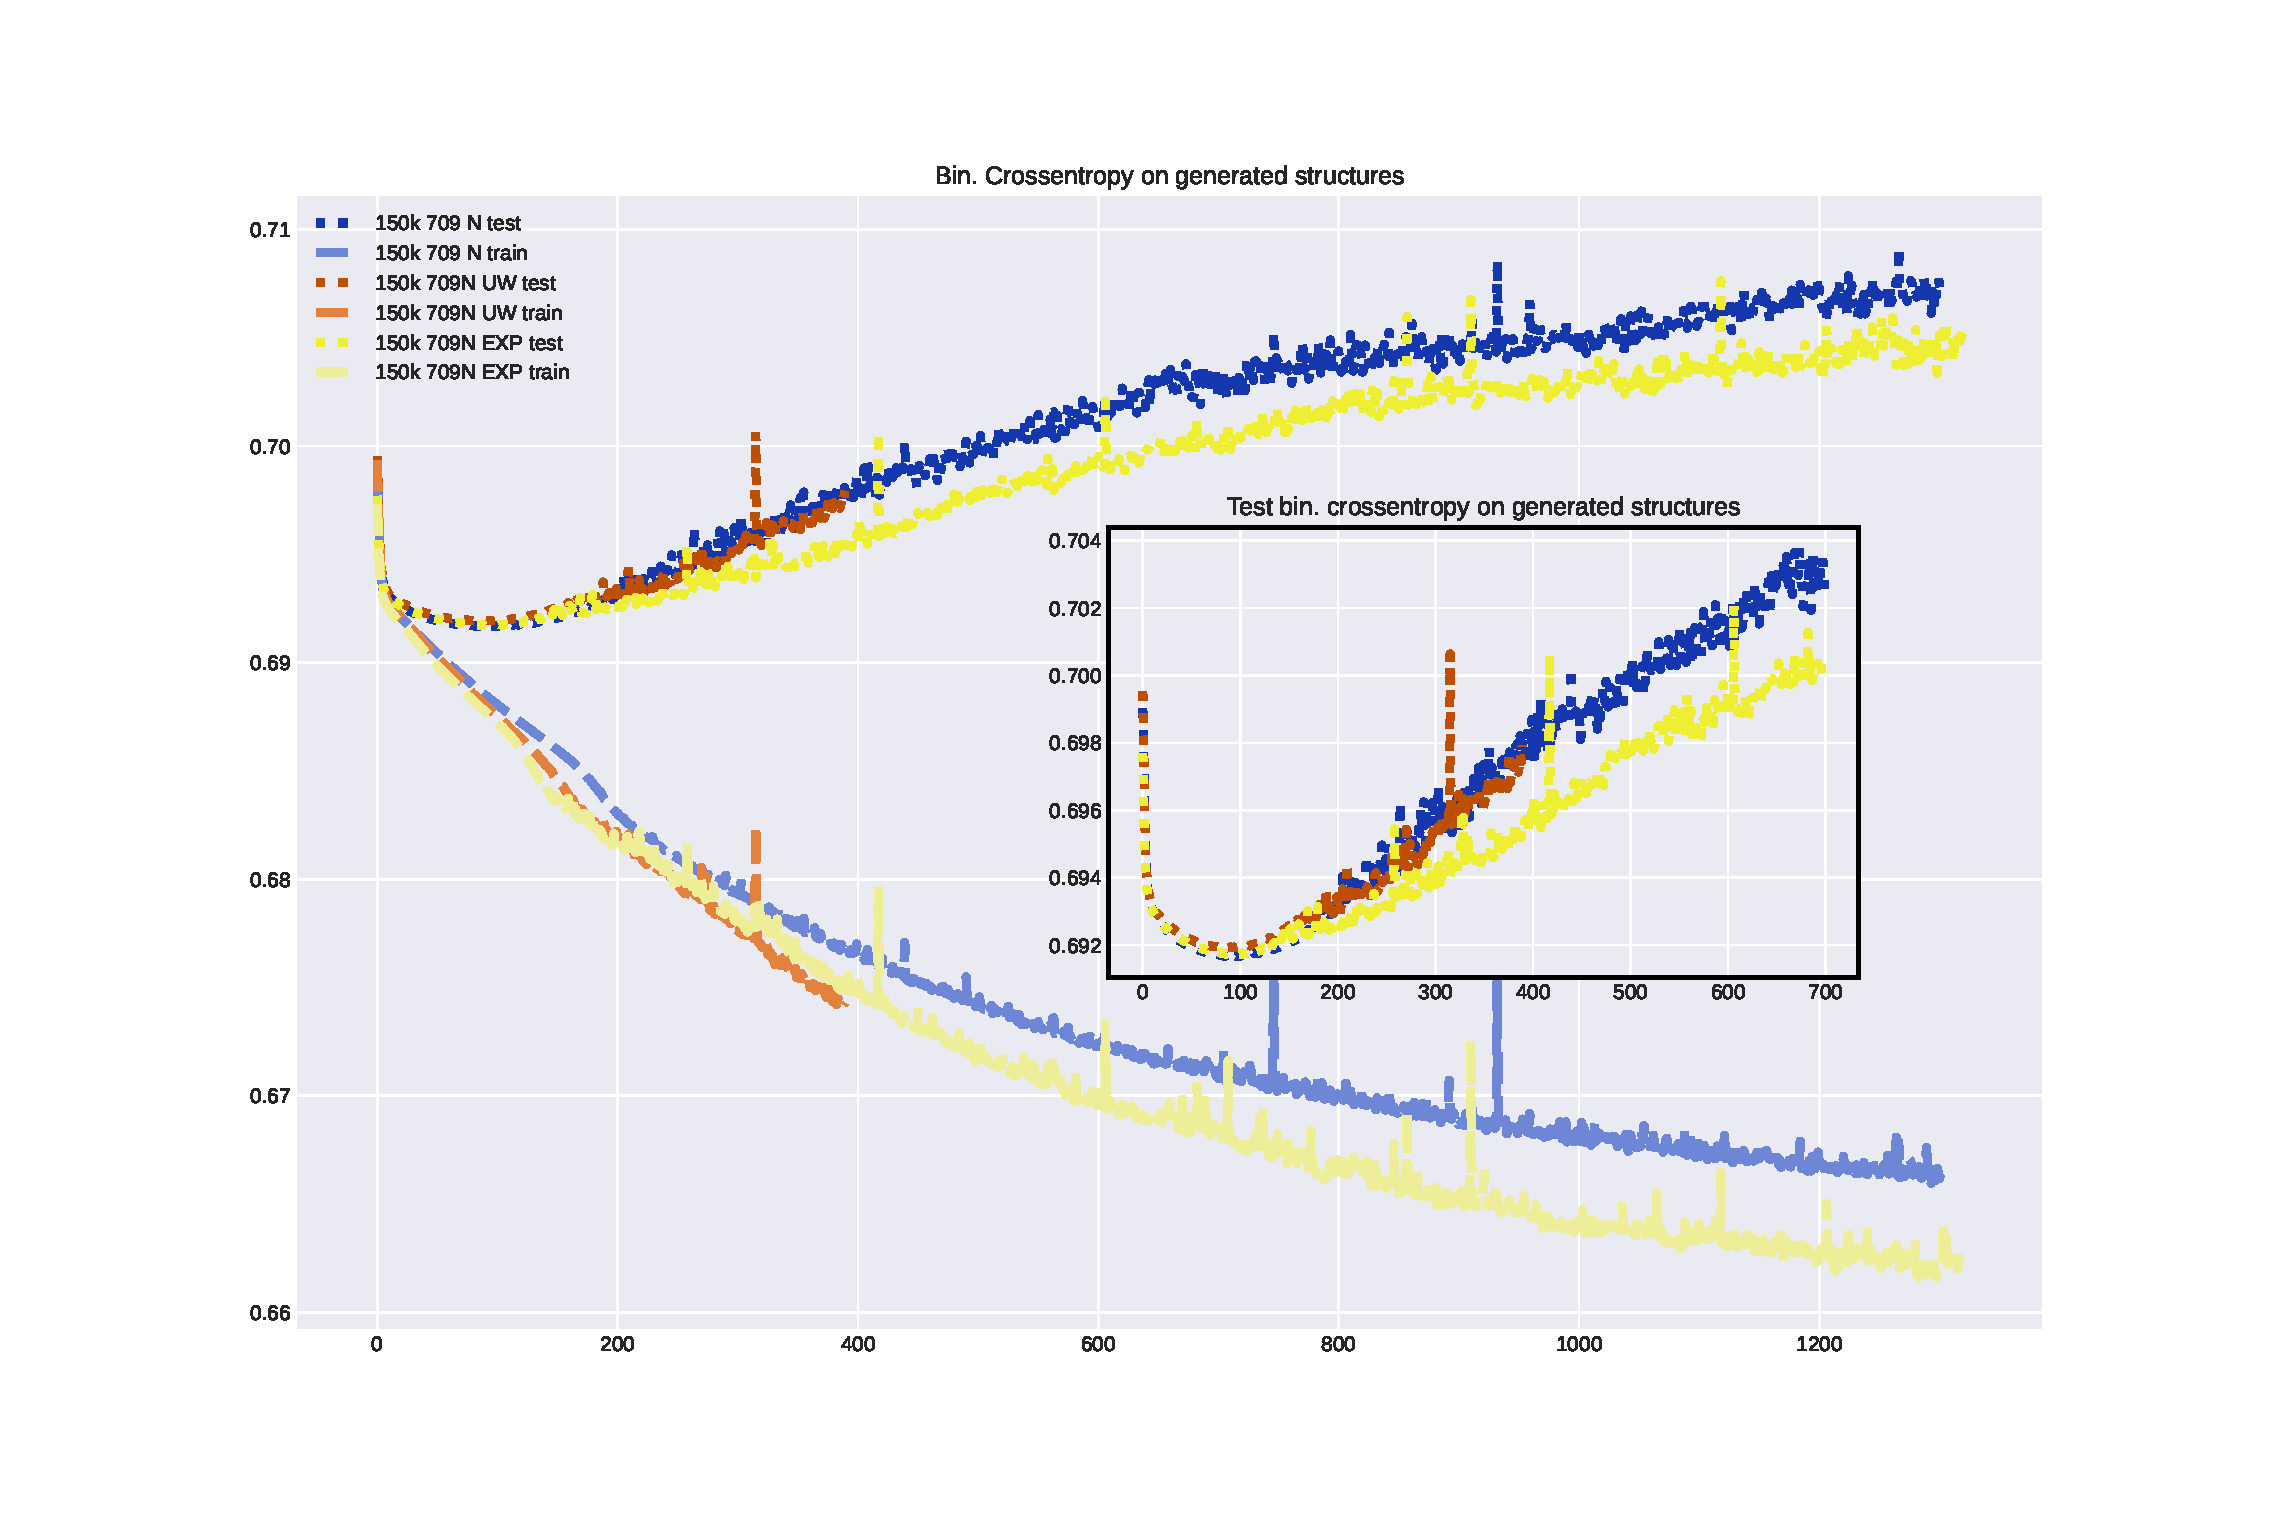
\includegraphics[width=\linewidth]{imgs/loss-weight.eps}
  \caption{Функция ошибки нейросети в зависимости от весов функции ошибки}\label{fig:loss_weight}
\endminipage
\end{figure}

Была исследована зависимость качества обучения от размера слоя нейросети для нейросети с 1 слоем. Полученные графики обучения (рис. \ref{fig:acc_lsize}, \ref{fig:loss_lsize}) говорят о том, что при уменьшении размера слоя с одной стороны снижается степень переобучения, с другой при уменьшении размера слоя до менее чем 100 нейронов происходит заметное снижение качества обучения. Таким образом, оптимальный размер скрытого слоя нейросети вероятно составляет 100 нейронов. Этот результат заставил нас провести исследование степени сжимаемости данных с помощью автокодировщика.

\begin{figure}[!h]
\minipage{0.5\textwidth}
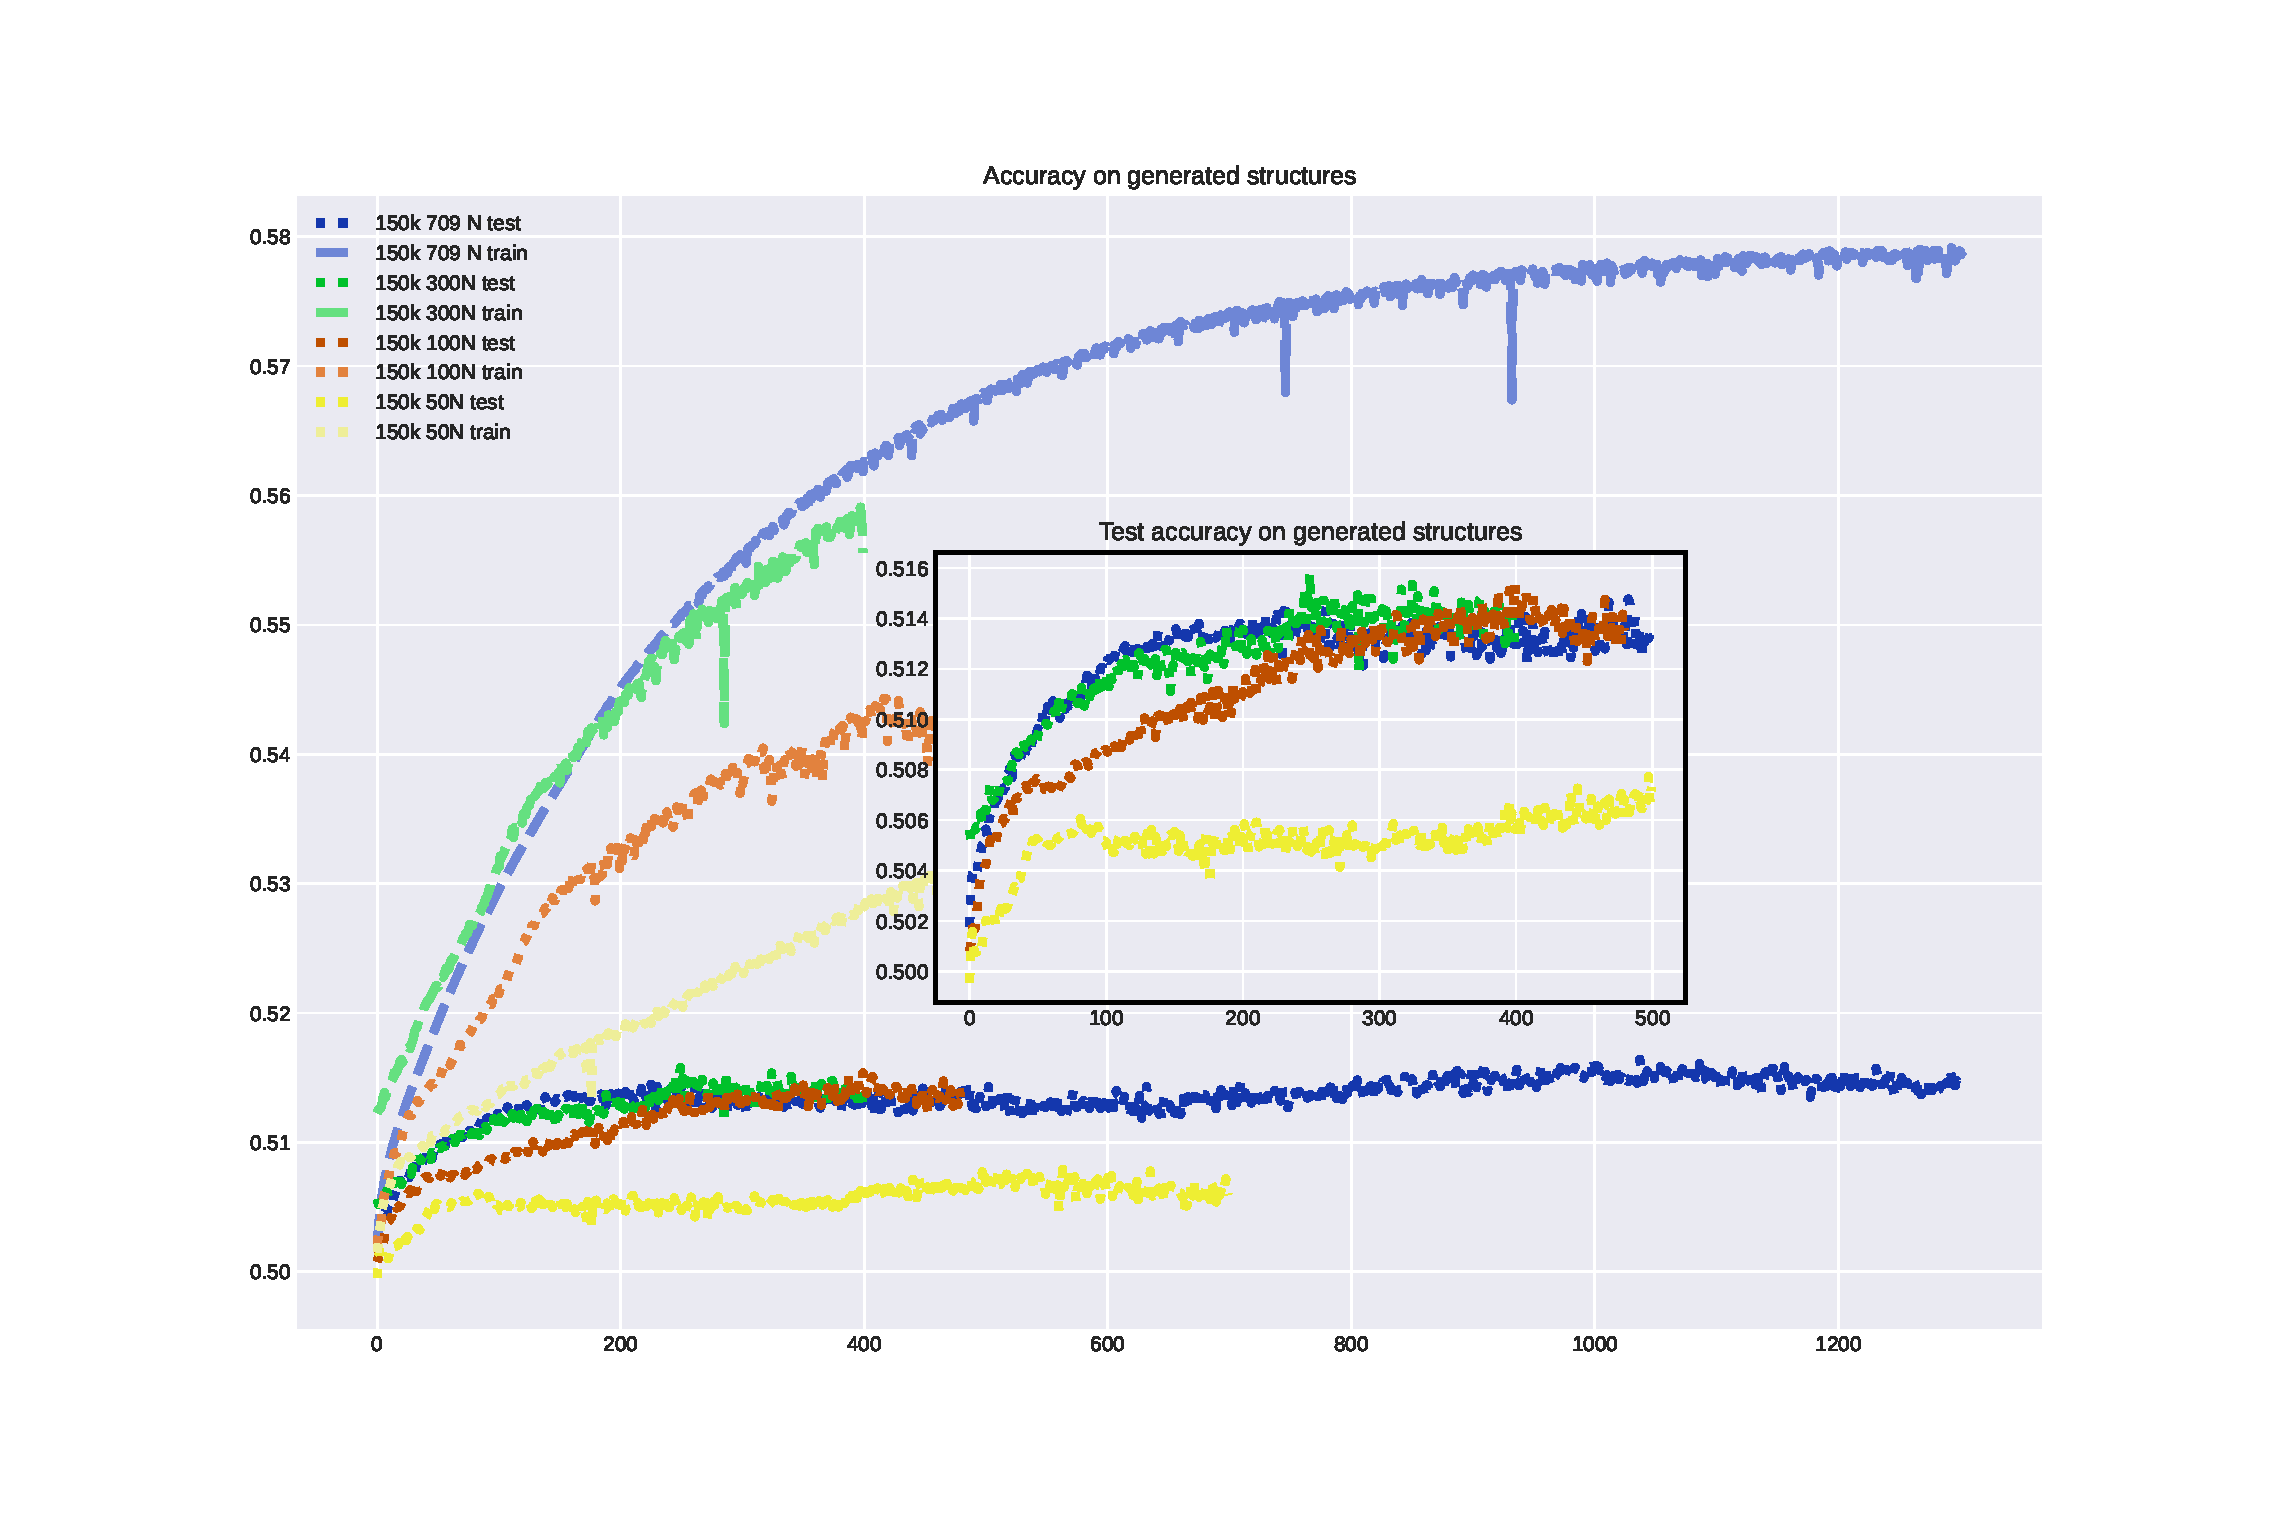
\includegraphics[width=\linewidth]{imgs/acc-lsize.eps}
  \caption{Точность нейросети в зависимости от размеров скрытого слоя}\label{fig:acc_lsize}
\endminipage\hfill
\minipage{0.5\textwidth}%
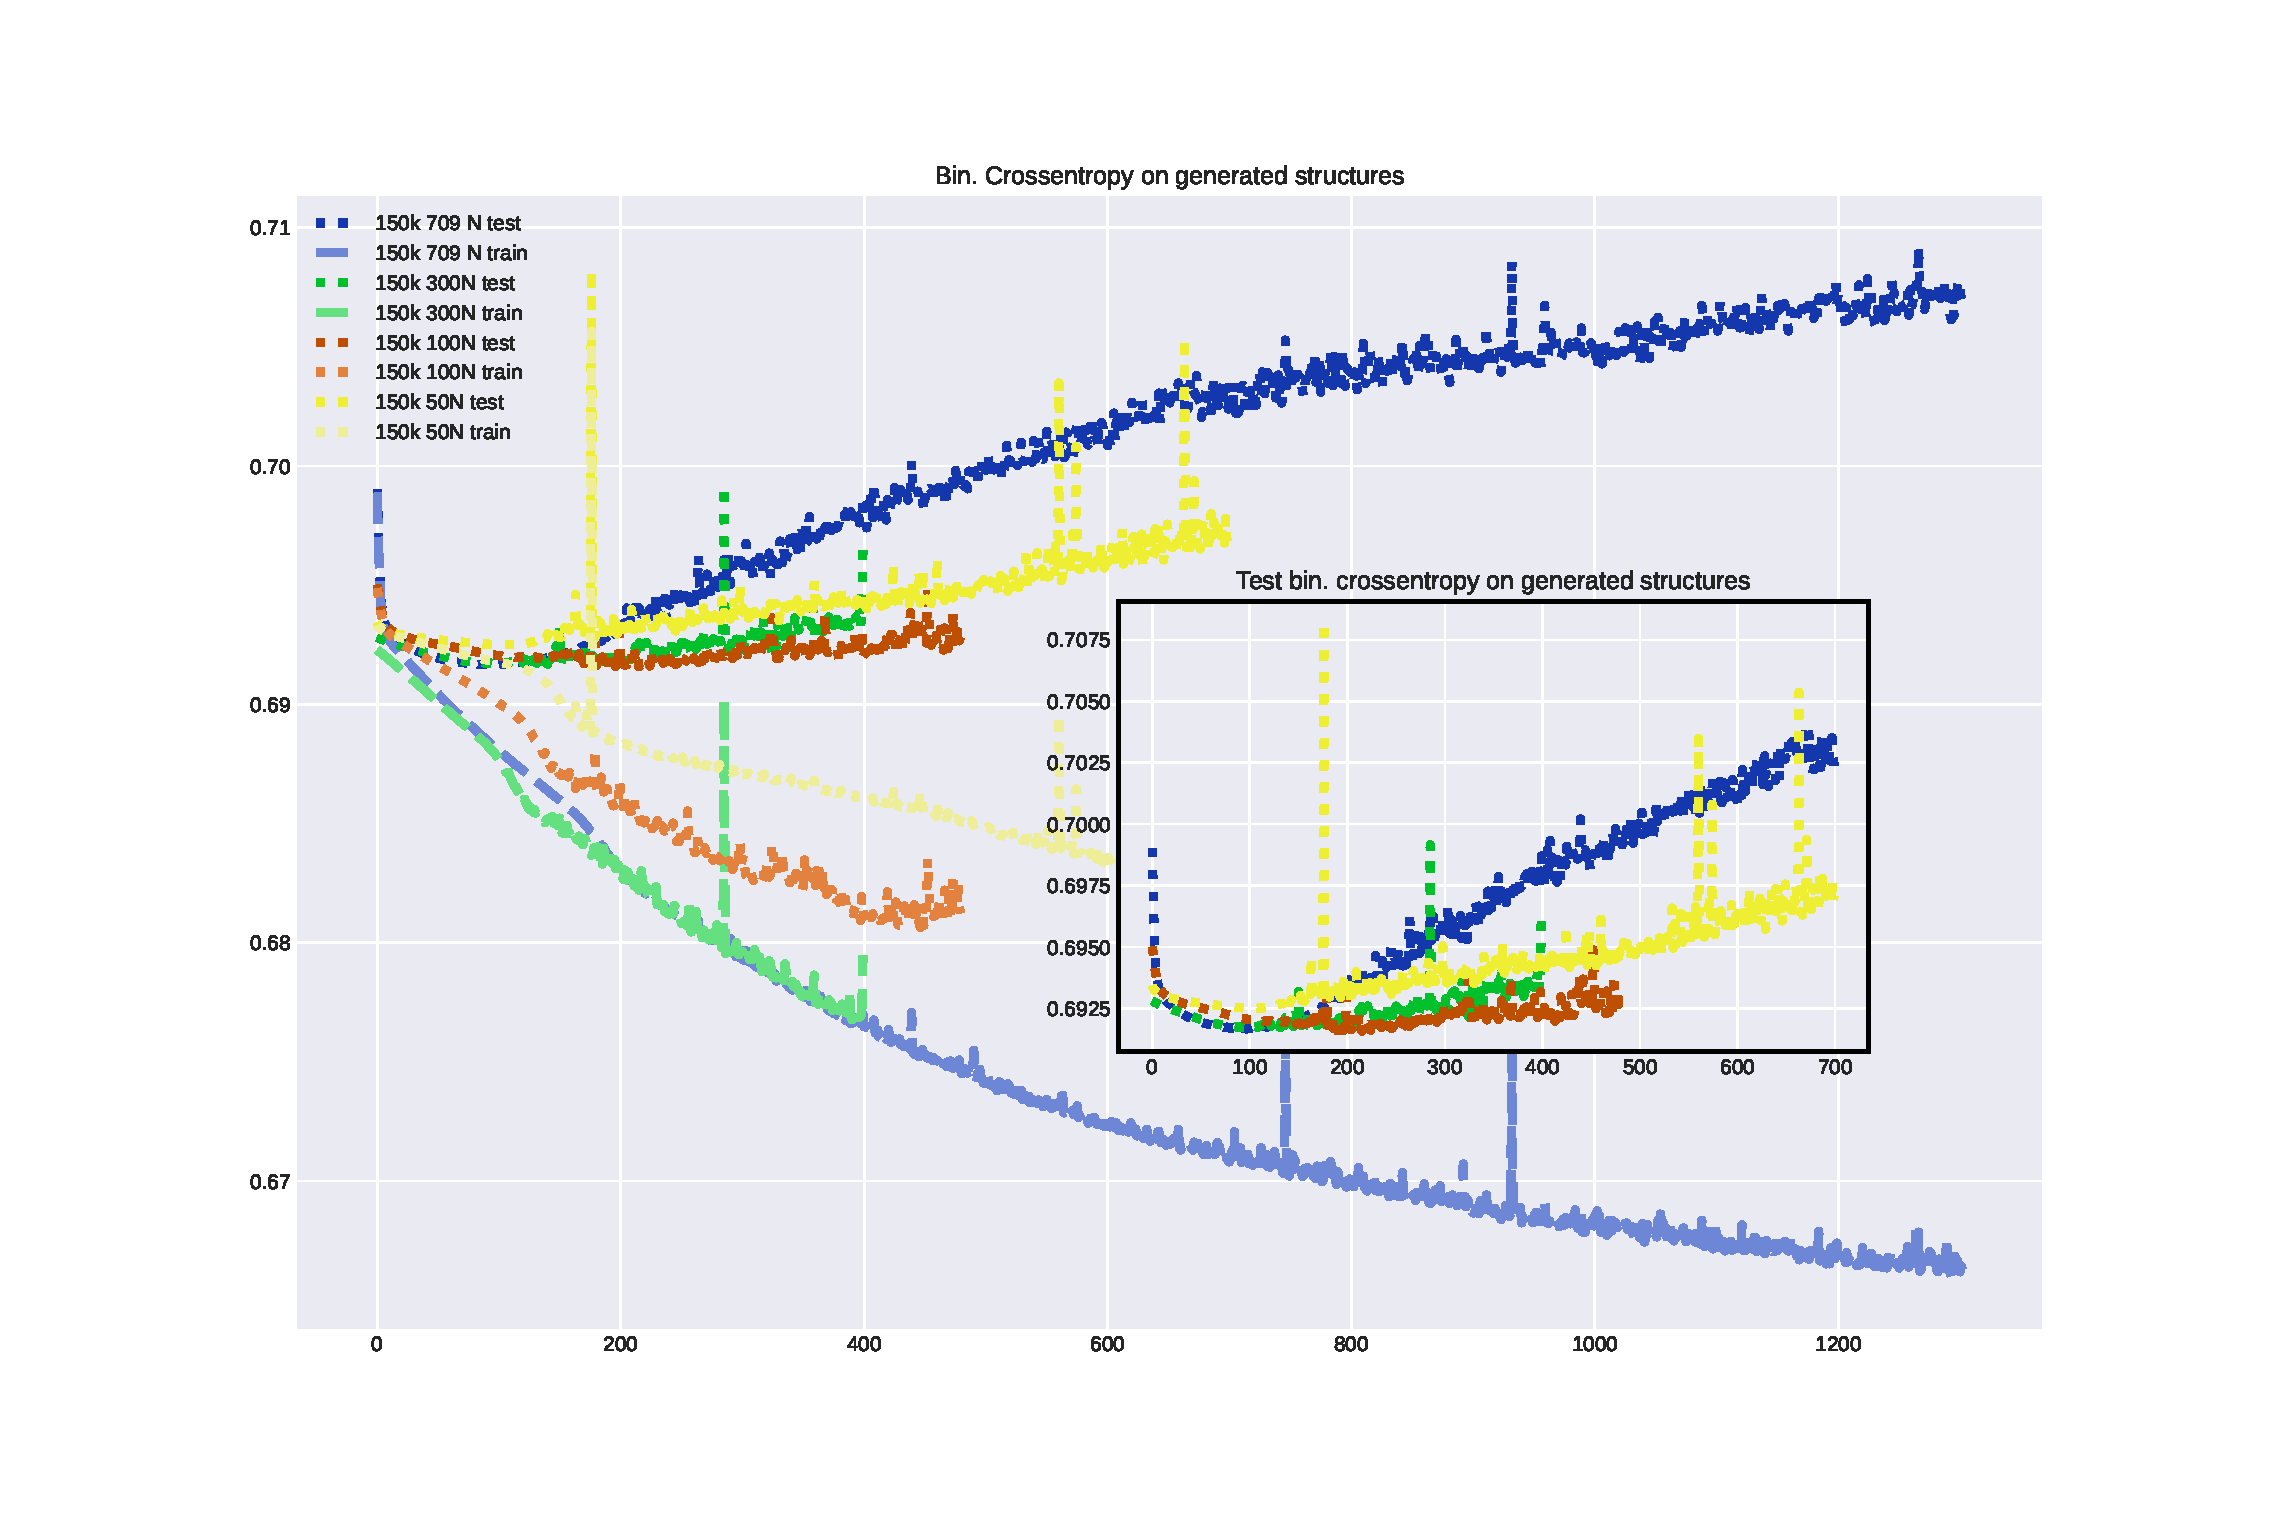
\includegraphics[width=\linewidth]{imgs/loss-lsize.eps}
  \caption{Функция ошибки нейросети в зависимости от размеров скрытого слоя}\label{fig:loss_lsize}
\endminipage
\end{figure}

\subsection{Применение автокодировщиков для определения сжимаемости данных}

Автокодировщик - нейронная сеть, задачей которой является получить на выходном слое нейрнонов значения максимально близкие к соответствующим значениям входного слоя. При этом промежуточный слой такой нейронной сети меньше, чем входной и выходной слои. Это заставляет нейросеть анализировать закономерности данных, выделять в них паттерны, т.е. сжимать данные. Таким образом по минимальному числу нейронов в скрытом слое с которым автокодировщик будет достаточно точно восстанавливать данные можно оценить количество информации на самом деле содержащееся в данных, которое в свою очередь определяет степень возможного сжатия данных и достаточный размер скрытых слоев нейронной сети.

Были обучены автокодировщики с размером скрытого слоя 50, 100, 250, 500, 1000 нейронов. Обучение проводилось без отброса дальних отражений, т.о. размер входа нейросети составил 4630 отражений на файл. Поскольку значения выходного слоя больше не являются бинарными, вместо бинарной кросссэентропии в качестве функции ошибки была применена среднеквадратичная ошибка(MSE, mean squared error). Полученные результаты представлены на рис. \ref{fig:loss_aenc}. Видно что большее количество нейронов в скрытом слое дает большую точность, но при этом если точность при 50 и 100 нейронах в скрытом слое заметно различается, то различия точности между 500 и 1000 нейронами почти нулевое.

\begin{figure}[htp]
\centering
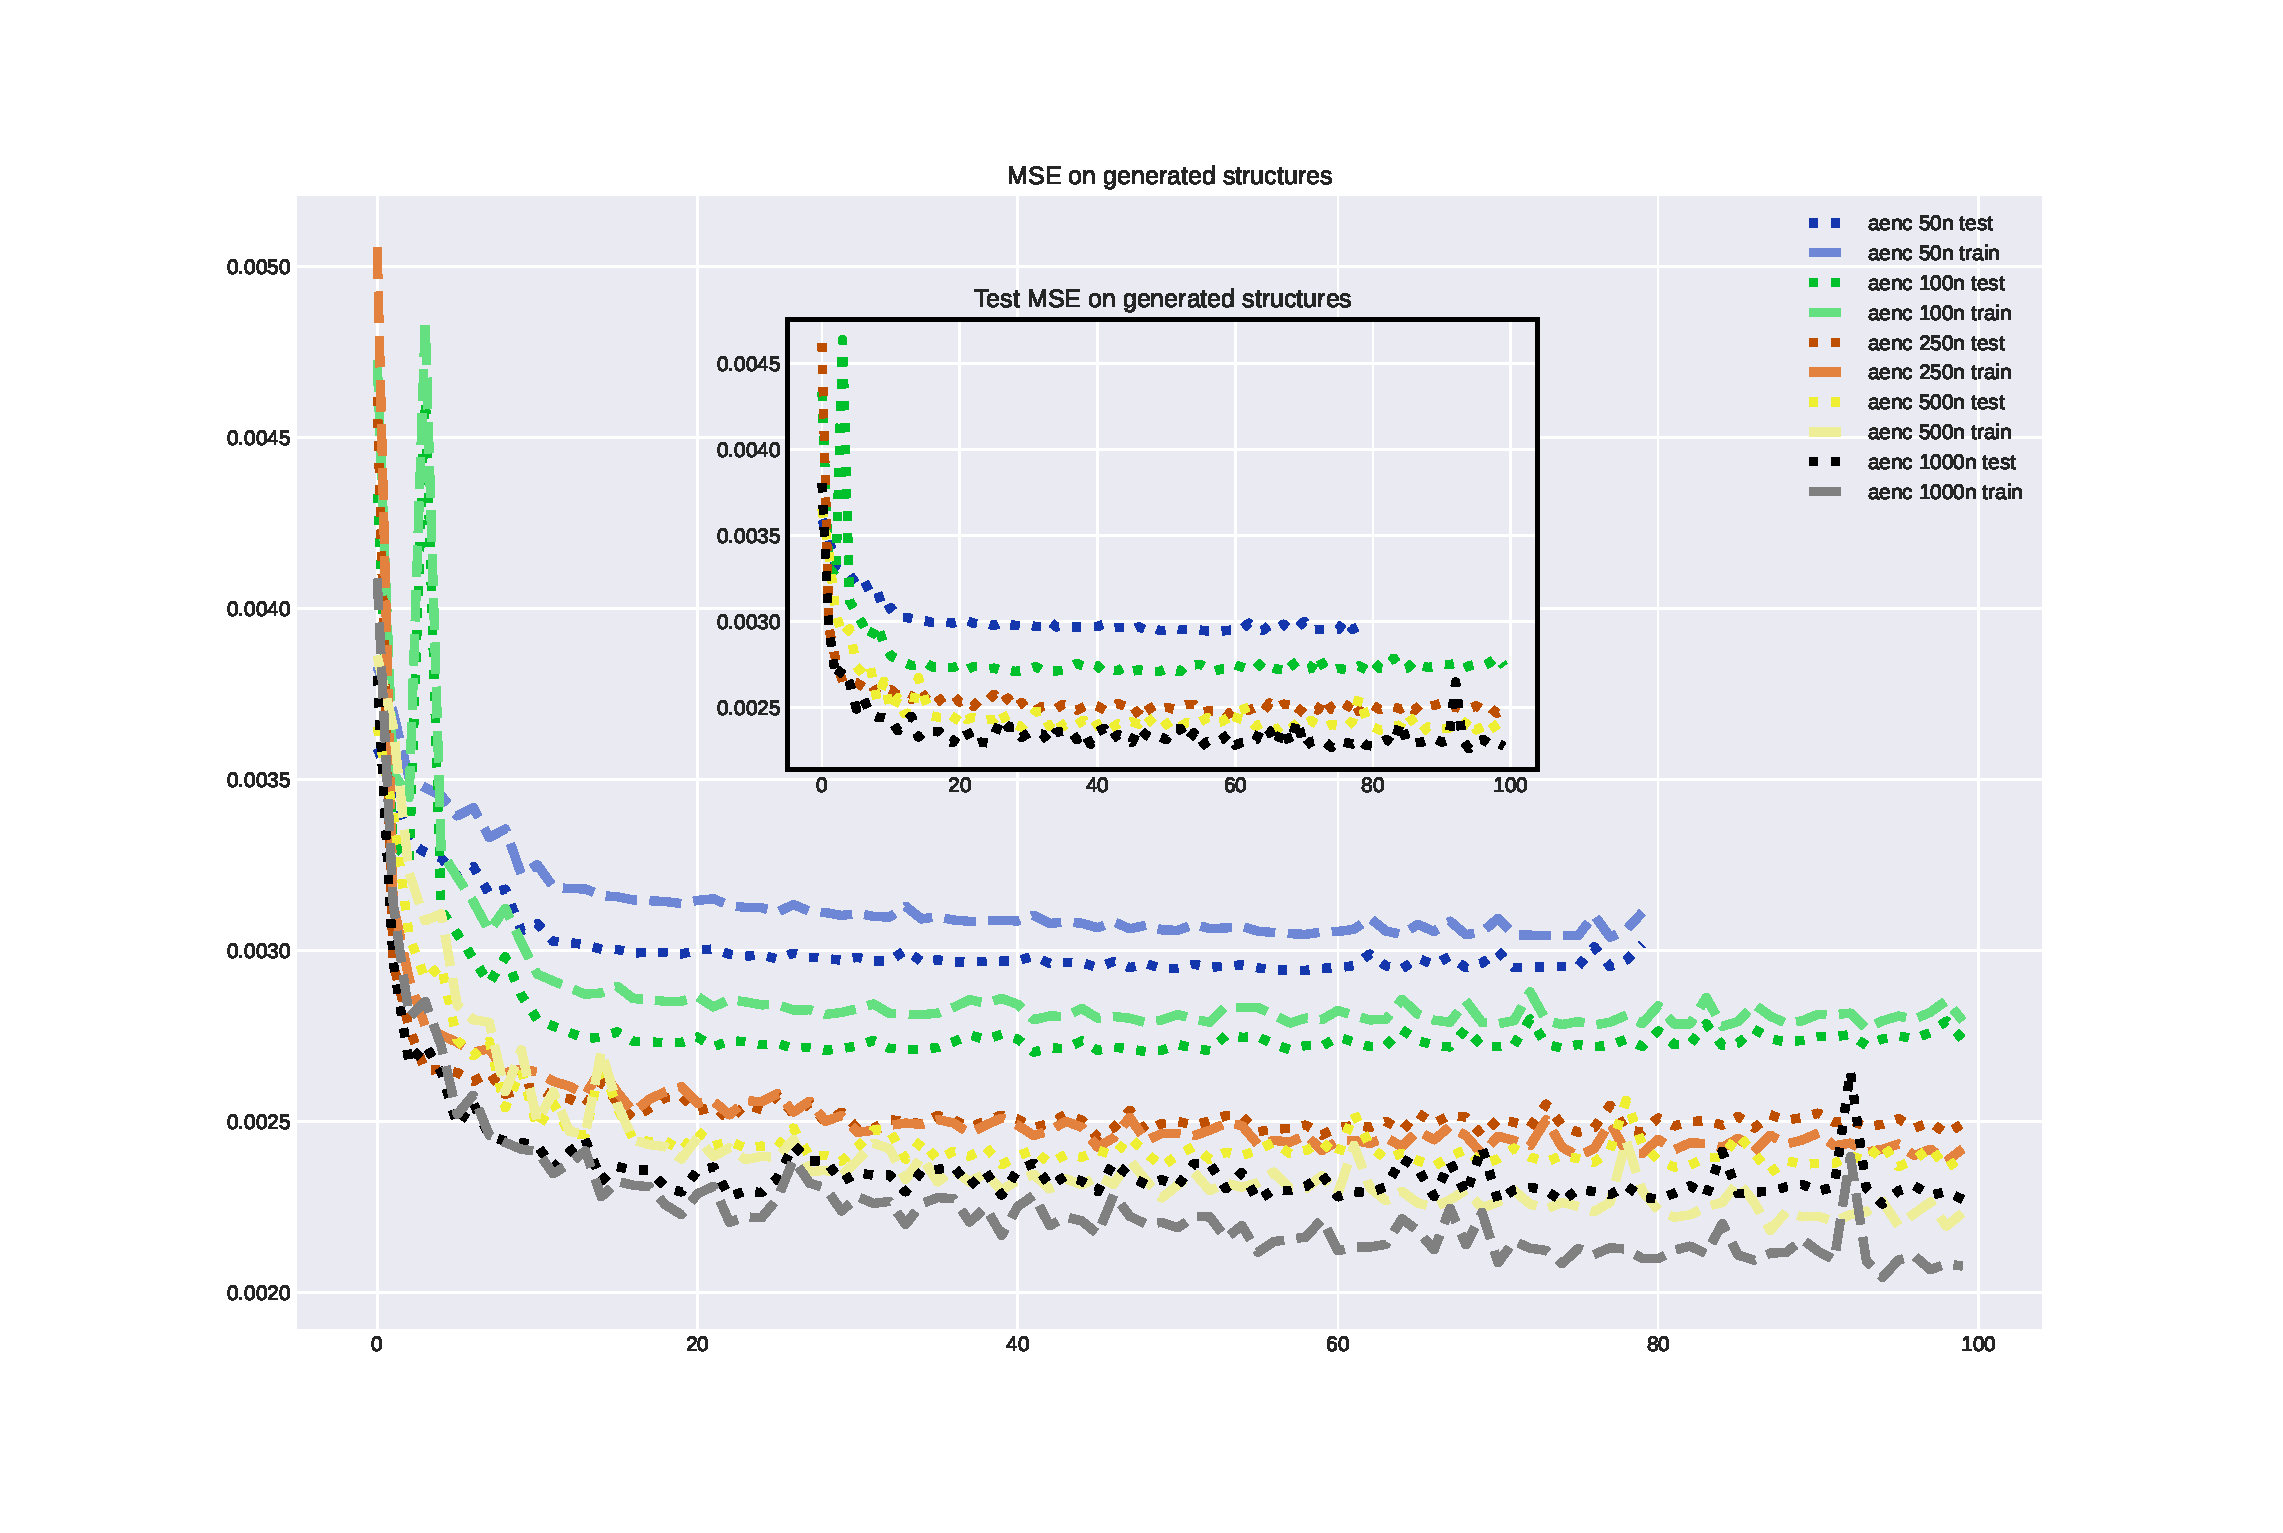
\includegraphics[scale=0.30]{imgs/loss-aenc.eps}
\caption{График обучения автоэнкодеров с разным размером скрытого слоя}
\label{fig:loss_aenc}
\end{figure}

Было проверено распределение ошибки по отражениям, результат представлен на рис. \ref{fig:aenc_errdist}, \ref{fig:aenc_errdist_fl}. Отражения на графиках отсортированы по $R=h^2+ k^2 + l^2, h,k,l$. На рис. \ref{fig:aenc_errdist_fl} применено сглаживание - показаны средние данные для окна в 50 точек. Видно что абсолютное значение среднеквадратичной ошибки выше для ближних, более интенсивных, отражений. Относительная ошибка для ближних отражений также чуть выше для малых $h,k,l$.

\begin{figure}[htp]
\centering
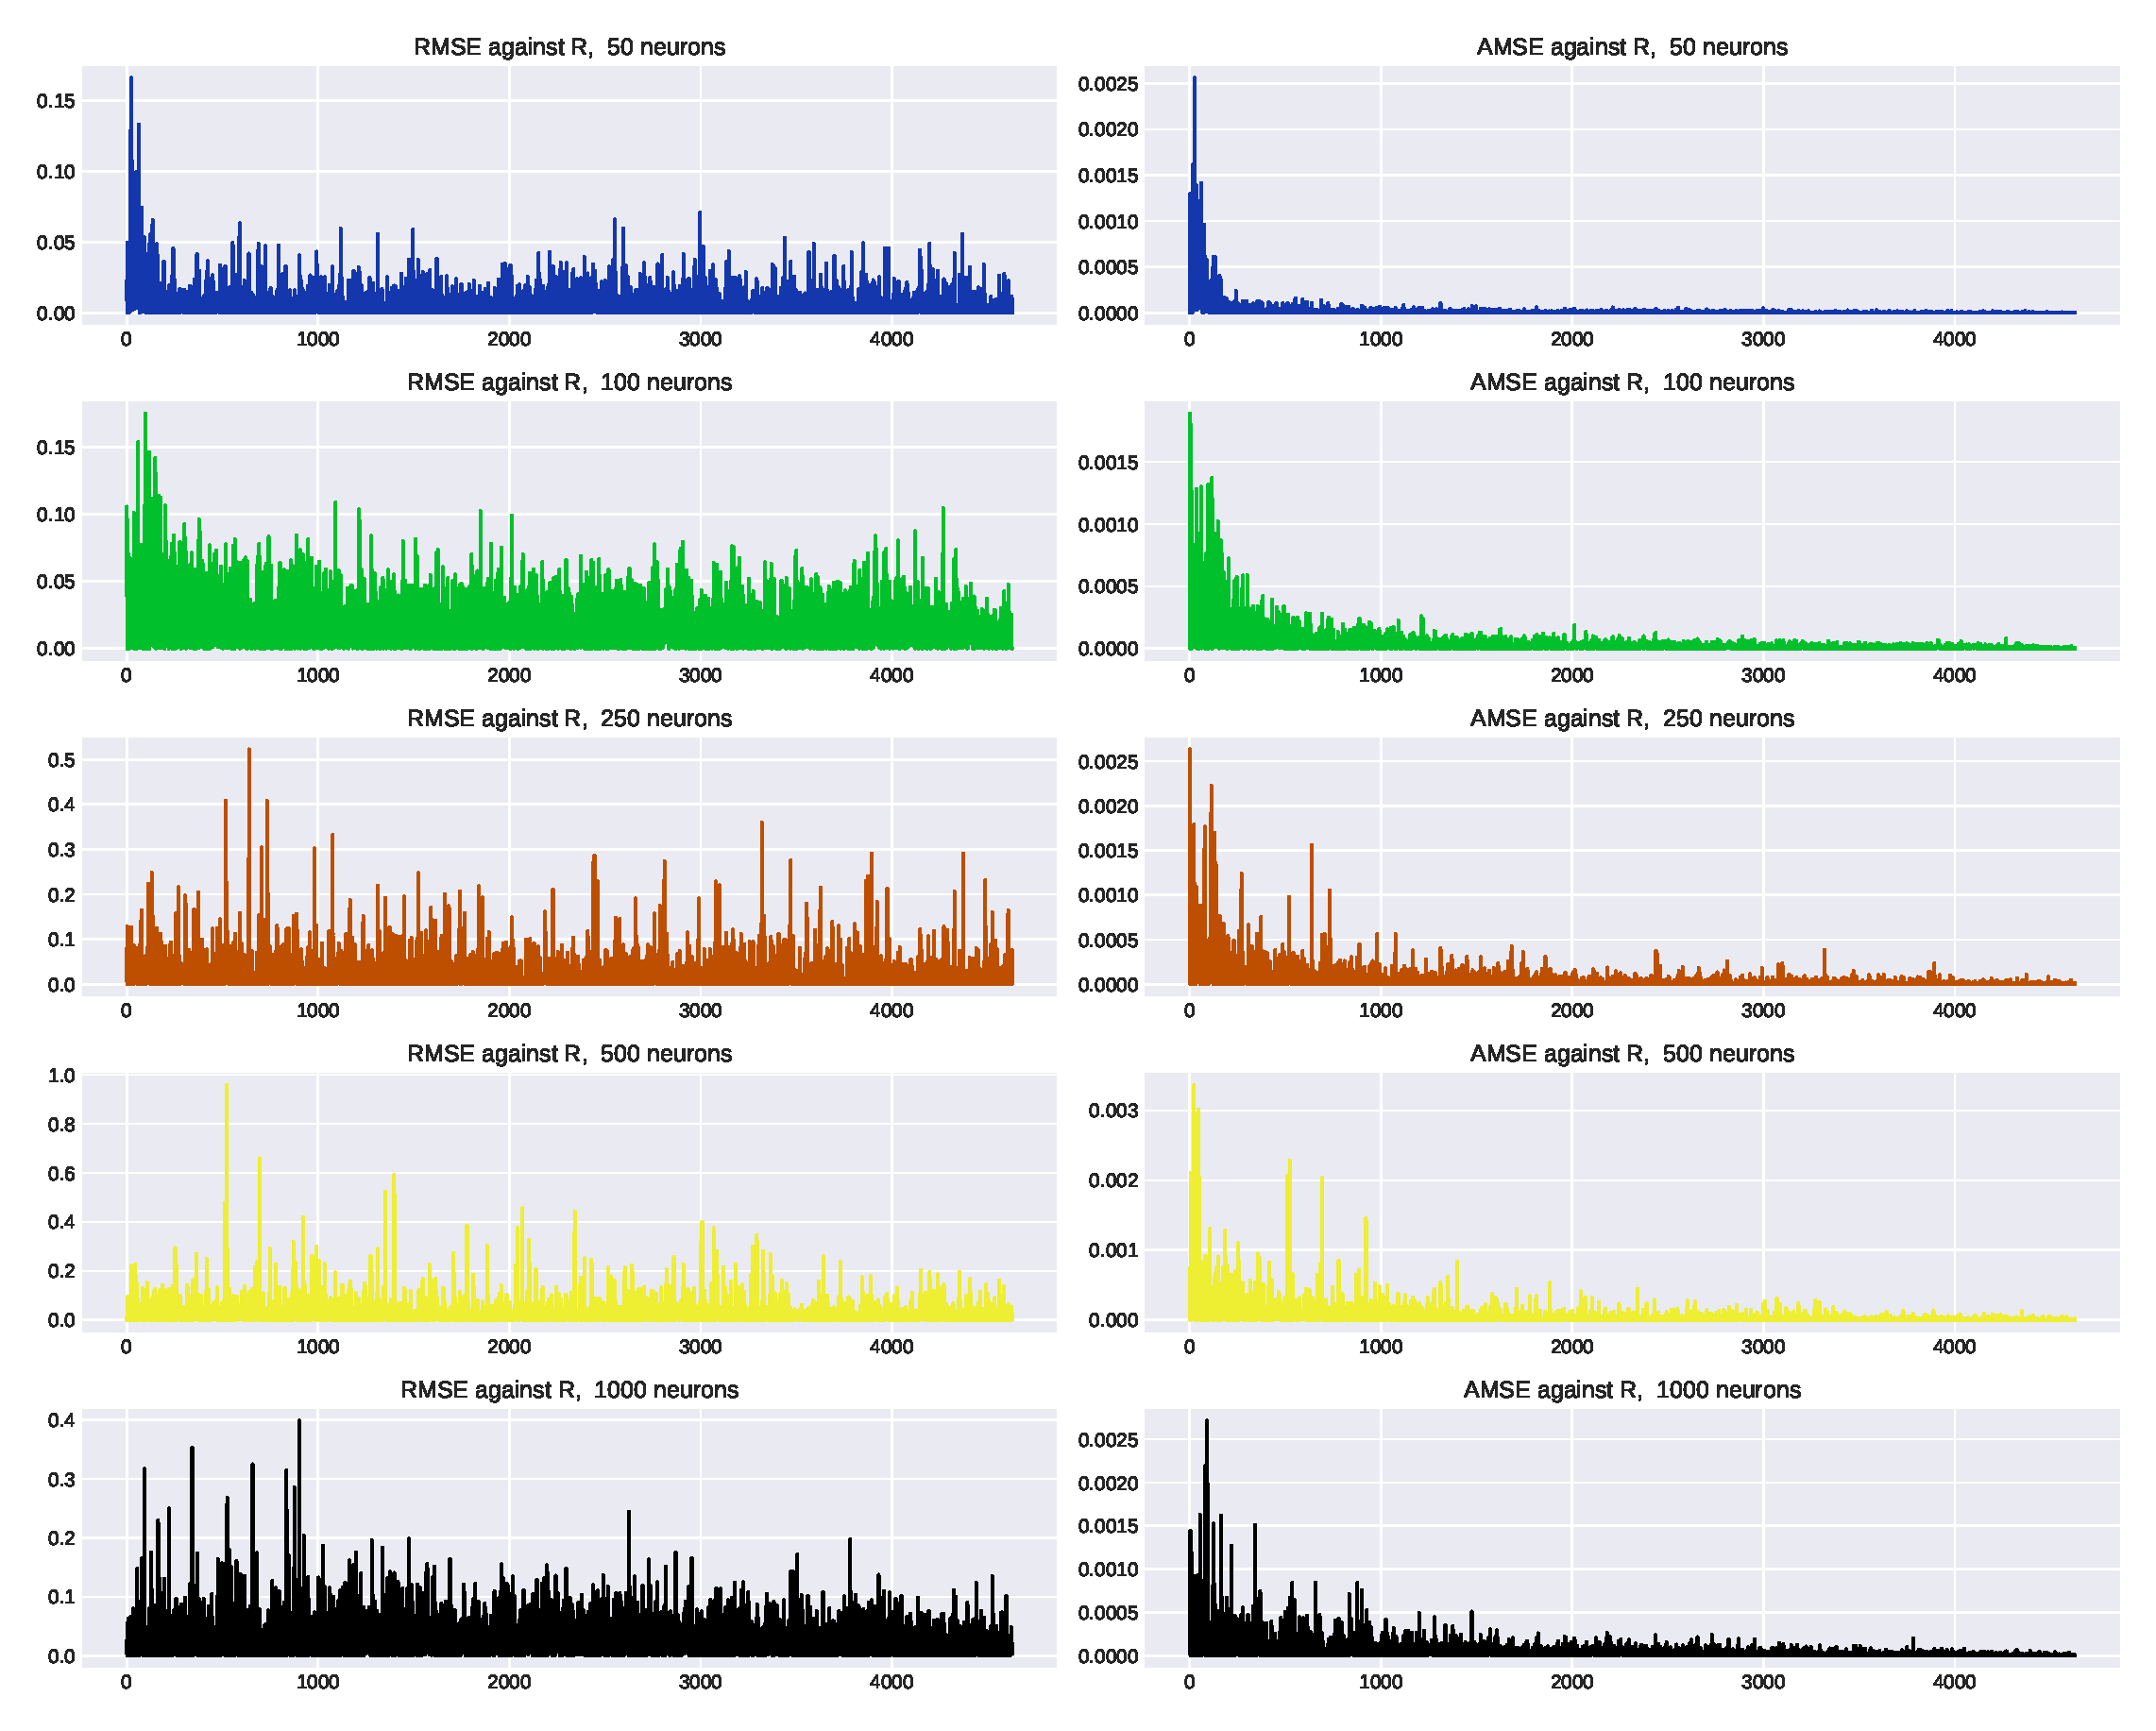
\includegraphics[width=\linewidth]{imgs/aenc-errdist.eps}
\caption{Распределение ошибки по отражениям}
\label{fig:aenc_errdist}
\end{figure}


\begin{figure}[htp]
\centering
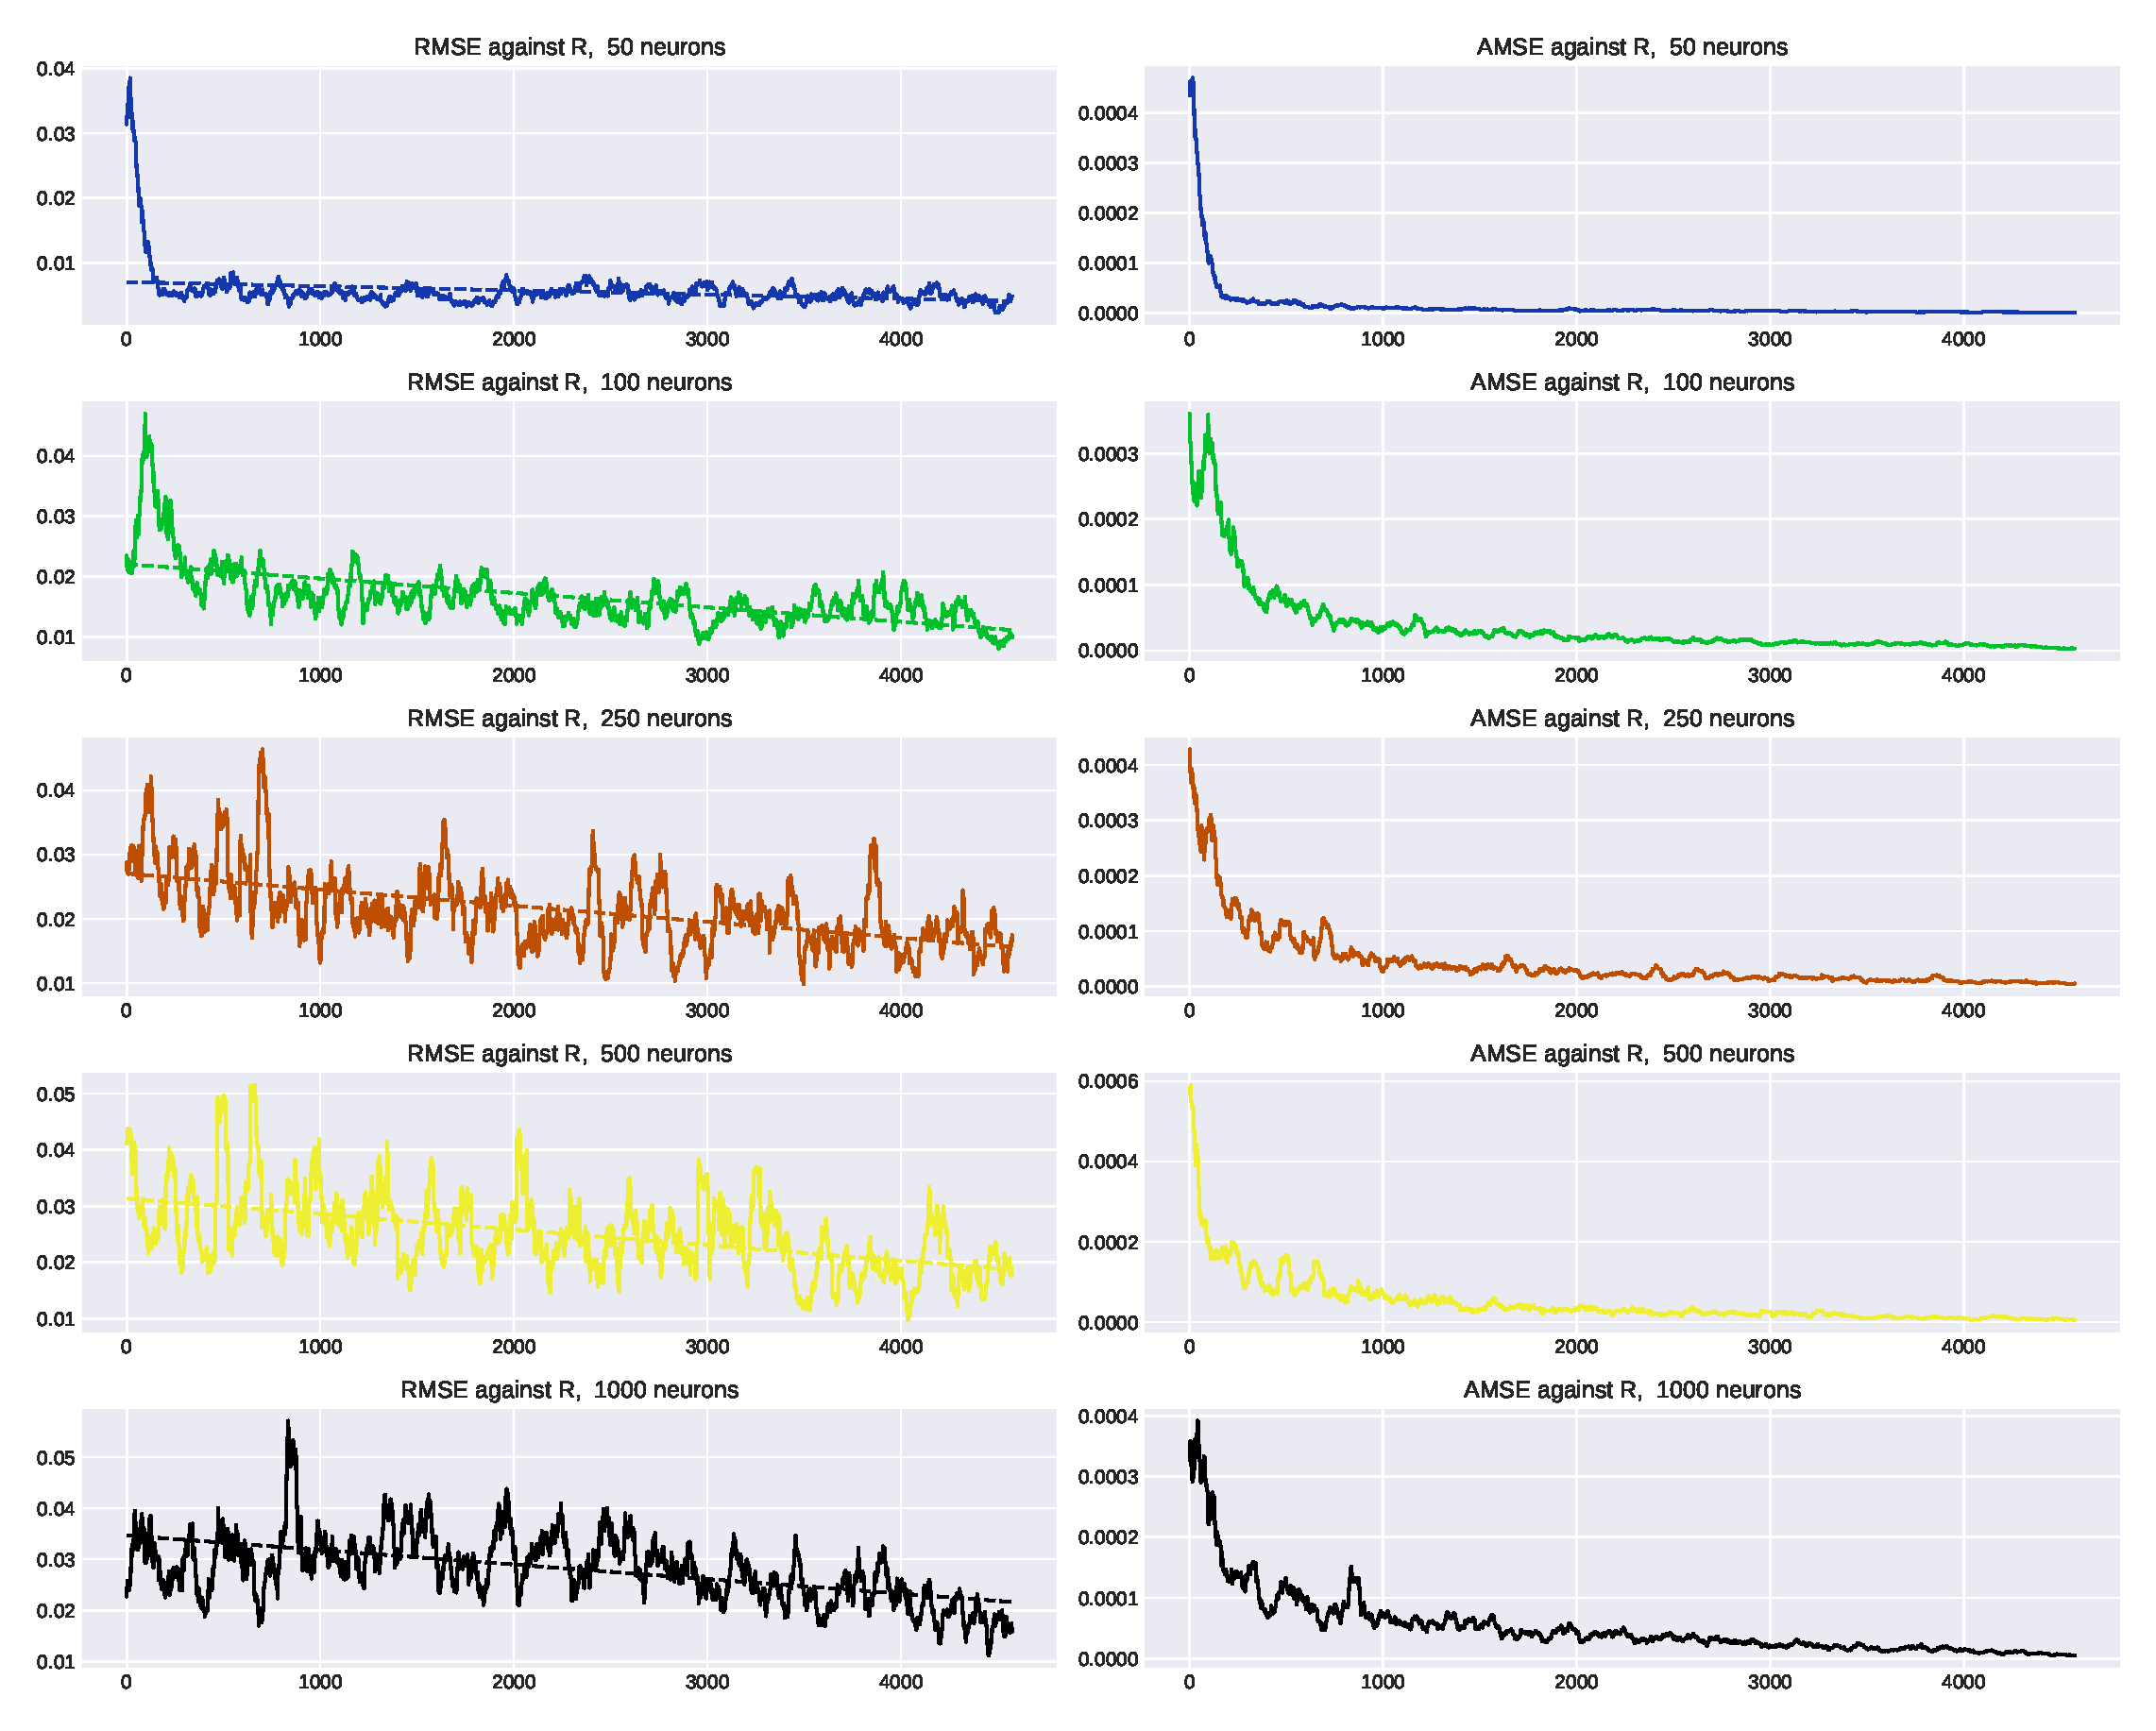
\includegraphics[scale=0.50]{imgs/aenc-errdist_fl.eps}
\caption{распределение ошибки по отражениям}
\label{fig:aenc_errdist_fl}
\end{figure}



%TODO 2k, 3, 4k, 10, 1

%Сравнить эксп. ошибку с автоэнкодерской

%Распеделение ошибок автоэнк/эксп

%Сравнить 




\section{РЕЗУЛЬТАТЫ И ВЫВОДЫ}

Были получены и обработаны кристаллографические данные. Построена модель машинного обучения для решения проблемы фаз для рентгеновских отражений, продемонстрировано серьезное переобучение. Это может быть объяснено тремя причинами:
\begin{itemize}
\item В интенсивностях отражений не содержится достаточно данных для определения фаз. В этом случае помочь может добавление параметров кристаллической решетки и других данных во входные данные нейронной сети
\item Недостаточно данных для обучения. В этом случае решить пробему поможет увеличение размеров датасета, например с помощью OQMD или путем аугментации датасета.
\item Нейронная сеть имеет слишком высокую запоминающую способность. В этом случае проблема может быть решена подбором оптимальной архитектуры: добавлением дропаутов, пакетных нормализаций, уменьшением размера слоев нейронной сети.
\end{itemize}
Еще одним вариантом улучшения результатов может быть использование вместо интенсивностей функции паттерсона\cite{PattersonMethod} - картины электронной плотности полученной исходя из предположения о том что фазы всех отражений идентичны и равны нулю. 

\printbibliography


\end{document}
